\documentclass[../main.tex]{subfiles}

\begin{document}
    \subsubsection*{Uncertainties}
        Every following uncertainty was calculated using this formula
        \[u:=\fdef{\fdef{\sqrt{\sum_{i\in\text{Def}(x)}\diff{f}{u(x_i)}{x}{}}}{x\in\text{Def}{f}}}{f\in C^(\R^d,\R)}.\]
		        
        
    \subsection{Isentropric Exponent}

    \subsection{Degrees of freedom}
        We firstly deduce the following plots from our data. 
        %\begin{figure}[H]

	\centering
	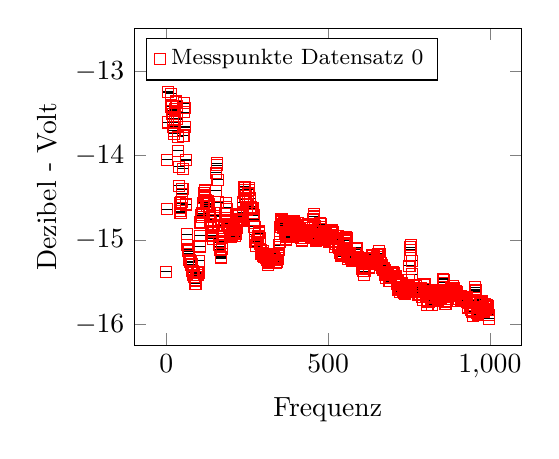
\begin{tikzpicture}
		\pgfplotsset{width=6.5cm,compat=1.3,legend style={font=\footnotesize}}
		\begin{axis}[xlabel={Frequenz},ylabel={Dezibel - Volt},legend cell align=left,legend pos=north west]
		
\addplot+[only marks,color=red,mark=square,error bars/.cd,x dir=both,x explicit,y dir=both,y explicit,error bar style={color=black}] table[x=X,y=Y,x error=xerror,y error=yerror,row sep=\\]{
			X	Y	xerror	yerror	\\
			 0.0 	 -15.377863 	 0 	 0 	\\
			 1.464844 	 -14.634824 	 0 	 0 	\\
			 2.929687 	 -14.048924 	 0 	 0 	\\
			 4.394531 	 -13.606714 	 0 	 0 	\\
			 5.859375 	 -13.245078 	 0 	 0 	\\
			 7.324219 	 -12.971722 	 0 	 0 	\\
			 8.789062 	 -12.828342 	 0 	 0 	\\
			 10.253906 	 -12.80232 	 0 	 0 	\\
			 11.71875 	 -12.891995 	 0 	 0 	\\
			 13.183594 	 -13.047378 	 0 	 0 	\\
			 14.648437 	 -13.266726 	 0 	 0 	\\
			 16.113281 	 -13.417296 	 0 	 0 	\\
			 17.578125 	 -13.467953 	 0 	 0 	\\
			 19.042969 	 -13.510851 	 0 	 0 	\\
			 20.507812 	 -13.562329 	 0 	 0 	\\
			 21.972656 	 -13.65778 	 0 	 0 	\\
			 23.4375 	 -13.742413 	 0 	 0 	\\
			 24.902344 	 -13.70612 	 0 	 0 	\\
			 26.367187 	 -13.603597 	 0 	 0 	\\
			 27.832031 	 -13.452496 	 0 	 0 	\\
			 29.296875 	 -13.360224 	 0 	 0 	\\
			 30.761719 	 -13.347933 	 0 	 0 	\\
			 32.226562 	 -13.416004 	 0 	 0 	\\
			 33.691406 	 -13.565305 	 0 	 0 	\\
			 35.15625 	 -13.777465 	 0 	 0 	\\
			 36.621094 	 -13.942297 	 0 	 0 	\\
			 38.085937 	 -14.13413 	 0 	 0 	\\
			 39.550781 	 -14.355808 	 0 	 0 	\\
			 41.015625 	 -14.567138 	 0 	 0 	\\
			 42.480469 	 -14.661787 	 0 	 0 	\\
			 43.945312 	 -14.676044 	 0 	 0 	\\
			 45.410156 	 -14.624667 	 0 	 0 	\\
			 46.875 	 -14.554264 	 0 	 0 	\\
			 48.339844 	 -14.454346 	 0 	 0 	\\
			 49.804687 	 -14.396066 	 0 	 0 	\\
			 51.269531 	 -14.157371 	 0 	 0 	\\
			 52.734375 	 -13.76188 	 0 	 0 	\\
			 54.199219 	 -13.486916 	 0 	 0 	\\
			 55.664062 	 -13.378995 	 0 	 0 	\\
			 57.128906 	 -13.436821 	 0 	 0 	\\
			 58.59375 	 -13.660917 	 0 	 0 	\\
			 60.058594 	 -14.051488 	 0 	 0 	\\
			 61.523437 	 -14.579972 	 0 	 0 	\\
			 62.988281 	 -14.932836 	 0 	 0 	\\
			 64.453125 	 -15.057708 	 0 	 0 	\\
			 65.917969 	 -15.10667 	 0 	 0 	\\
			 67.382812 	 -15.131666 	 0 	 0 	\\
			 68.847656 	 -15.120015 	 0 	 0 	\\
			 70.3125 	 -15.166563 	 0 	 0 	\\
			 71.777344 	 -15.234852 	 0 	 0 	\\
			 73.242187 	 -15.257725 	 0 	 0 	\\
			 74.707031 	 -15.258081 	 0 	 0 	\\
			 76.171875 	 -15.262162 	 0 	 0 	\\
			 77.636719 	 -15.292419 	 0 	 0 	\\
			 79.101562 	 -15.302074 	 0 	 0 	\\
			 80.566406 	 -15.371643 	 0 	 0 	\\
			 82.03125 	 -15.414623 	 0 	 0 	\\
			 83.496094 	 -15.384488 	 0 	 0 	\\
			 84.960937 	 -15.38654 	 0 	 0 	\\
			 86.425781 	 -15.435651 	 0 	 0 	\\
			 87.890625 	 -15.480934 	 0 	 0 	\\
			 89.355469 	 -15.519261 	 0 	 0 	\\
			 90.820312 	 -15.520492 	 0 	 0 	\\
			 92.285156 	 -15.435193 	 0 	 0 	\\
			 93.75 	 -15.419489 	 0 	 0 	\\
			 95.214844 	 -15.394684 	 0 	 0 	\\
			 96.679687 	 -15.392082 	 0 	 0 	\\
			 98.144531 	 -15.417509 	 0 	 0 	\\
			 99.609375 	 -15.390234 	 0 	 0 	\\
			 101.074219 	 -15.246798 	 0 	 0 	\\
			 102.539062 	 -15.077027 	 0 	 0 	\\
			 104.003906 	 -14.951796 	 0 	 0 	\\
			 105.46875 	 -14.793155 	 0 	 0 	\\
			 106.933594 	 -14.725076 	 0 	 0 	\\
			 108.398437 	 -14.70885 	 0 	 0 	\\
			 109.863281 	 -14.729992 	 0 	 0 	\\
			 111.328125 	 -14.683022 	 0 	 0 	\\
			 112.792969 	 -14.633574 	 0 	 0 	\\
			 114.257812 	 -14.559146 	 0 	 0 	\\
			 115.722656 	 -14.497235 	 0 	 0 	\\
			 117.1875 	 -14.442762 	 0 	 0 	\\
			 118.652344 	 -14.413613 	 0 	 0 	\\
			 120.117187 	 -14.473501 	 0 	 0 	\\
			 121.582031 	 -14.529763 	 0 	 0 	\\
			 123.046875 	 -14.572319 	 0 	 0 	\\
			 124.511719 	 -14.599137 	 0 	 0 	\\
			 125.976562 	 -14.57376 	 0 	 0 	\\
			 127.441406 	 -14.5452 	 0 	 0 	\\
			 128.90625 	 -14.577725 	 0 	 0 	\\
			 130.371094 	 -14.570568 	 0 	 0 	\\
			 131.835937 	 -14.606959 	 0 	 0 	\\
			 133.300781 	 -14.677834 	 0 	 0 	\\
			 134.765625 	 -14.72607 	 0 	 0 	\\
			 136.230469 	 -14.783752 	 0 	 0 	\\
			 137.695312 	 -14.845978 	 0 	 0 	\\
			 139.160156 	 -14.890022 	 0 	 0 	\\
			 140.625 	 -14.942508 	 0 	 0 	\\
			 142.089844 	 -14.958278 	 0 	 0 	\\
			 143.554687 	 -14.984087 	 0 	 0 	\\
			 145.019531 	 -14.907987 	 0 	 0 	\\
			 146.484375 	 -14.833804 	 0 	 0 	\\
			 147.949219 	 -14.760233 	 0 	 0 	\\
			 149.414062 	 -14.716789 	 0 	 0 	\\
			 150.878906 	 -14.612332 	 0 	 0 	\\
			 152.34375 	 -14.415131 	 0 	 0 	\\
			 153.808594 	 -14.203882 	 0 	 0 	\\
			 155.273437 	 -14.090973 	 0 	 0 	\\
			 156.738281 	 -14.114061 	 0 	 0 	\\
			 158.203125 	 -14.28813 	 0 	 0 	\\
			 159.667969 	 -14.549723 	 0 	 0 	\\
			 161.132812 	 -14.826476 	 0 	 0 	\\
			 162.597656 	 -15.024029 	 0 	 0 	\\
			 164.0625 	 -15.059548 	 0 	 0 	\\
			 165.527344 	 -15.076732 	 0 	 0 	\\
			 166.992187 	 -15.118956 	 0 	 0 	\\
			 168.457031 	 -15.214337 	 0 	 0 	\\
			 169.921875 	 -15.197879 	 0 	 0 	\\
			 171.386719 	 -15.102572 	 0 	 0 	\\
			 172.851562 	 -15.033952 	 0 	 0 	\\
			 174.316406 	 -14.968841 	 0 	 0 	\\
			 175.78125 	 -14.886593 	 0 	 0 	\\
			 177.246094 	 -14.857826 	 0 	 0 	\\
			 178.710937 	 -14.834681 	 0 	 0 	\\
			 180.175781 	 -14.781653 	 0 	 0 	\\
			 181.640625 	 -14.697632 	 0 	 0 	\\
			 183.105469 	 -14.612491 	 0 	 0 	\\
			 184.570312 	 -14.565412 	 0 	 0 	\\
			 186.035156 	 -14.630101 	 0 	 0 	\\
			 187.5 	 -14.763068 	 0 	 0 	\\
			 188.964844 	 -14.81181 	 0 	 0 	\\
			 190.429687 	 -14.809167 	 0 	 0 	\\
			 191.894531 	 -14.820498 	 0 	 0 	\\
			 193.359375 	 -14.83837 	 0 	 0 	\\
			 194.824219 	 -14.842676 	 0 	 0 	\\
			 196.289062 	 -14.914527 	 0 	 0 	\\
			 197.753906 	 -14.937226 	 0 	 0 	\\
			 199.21875 	 -14.963659 	 0 	 0 	\\
			 200.683594 	 -14.964335 	 0 	 0 	\\
			 202.148437 	 -14.949748 	 0 	 0 	\\
			 203.613281 	 -14.918795 	 0 	 0 	\\
			 205.078125 	 -14.910389 	 0 	 0 	\\
			 206.542969 	 -14.885805 	 0 	 0 	\\
			 208.007812 	 -14.866659 	 0 	 0 	\\
			 209.472656 	 -14.877181 	 0 	 0 	\\
			 210.9375 	 -14.919722 	 0 	 0 	\\
			 212.402344 	 -14.957385 	 0 	 0 	\\
			 213.867187 	 -14.929474 	 0 	 0 	\\
			 215.332031 	 -14.902048 	 0 	 0 	\\
			 216.796875 	 -14.855239 	 0 	 0 	\\
			 218.261719 	 -14.814927 	 0 	 0 	\\
			 219.726562 	 -14.754177 	 0 	 0 	\\
			 221.191406 	 -14.698331 	 0 	 0 	\\
			 222.65625 	 -14.7121 	 0 	 0 	\\
			 224.121094 	 -14.720584 	 0 	 0 	\\
			 225.585937 	 -14.752912 	 0 	 0 	\\
			 227.050781 	 -14.754292 	 0 	 0 	\\
			 228.515625 	 -14.7607 	 0 	 0 	\\
			 229.980469 	 -14.754367 	 0 	 0 	\\
			 231.445312 	 -14.766731 	 0 	 0 	\\
			 232.910156 	 -14.774063 	 0 	 0 	\\
			 234.375 	 -14.75994 	 0 	 0 	\\
			 235.839844 	 -14.672699 	 0 	 0 	\\
			 237.304687 	 -14.553177 	 0 	 0 	\\
			 238.769531 	 -14.442574 	 0 	 0 	\\
			 240.234375 	 -14.380149 	 0 	 0 	\\
			 241.699219 	 -14.37053 	 0 	 0 	\\
			 243.164062 	 -14.405877 	 0 	 0 	\\
			 244.628906 	 -14.478126 	 0 	 0 	\\
			 246.09375 	 -14.525214 	 0 	 0 	\\
			 247.558594 	 -14.571617 	 0 	 0 	\\
			 249.023437 	 -14.640223 	 0 	 0 	\\
			 250.488281 	 -14.62722 	 0 	 0 	\\
			 251.953125 	 -14.545152 	 0 	 0 	\\
			 253.417969 	 -14.450371 	 0 	 0 	\\
			 254.882812 	 -14.385941 	 0 	 0 	\\
			 256.347656 	 -14.403229 	 0 	 0 	\\
			 257.8125 	 -14.507634 	 0 	 0 	\\
			 259.277344 	 -14.623046 	 0 	 0 	\\
			 260.742187 	 -14.619449 	 0 	 0 	\\
			 262.207031 	 -14.607496 	 0 	 0 	\\
			 263.671875 	 -14.6373 	 0 	 0 	\\
			 265.136719 	 -14.621309 	 0 	 0 	\\
			 266.601562 	 -14.623232 	 0 	 0 	\\
			 268.066406 	 -14.675993 	 0 	 0 	\\
			 269.53125 	 -14.705281 	 0 	 0 	\\
			 270.996094 	 -14.7643 	 0 	 0 	\\
			 272.460937 	 -14.844184 	 0 	 0 	\\
			 273.925781 	 -14.933865 	 0 	 0 	\\
			 275.390625 	 -15.023675 	 0 	 0 	\\
			 276.855469 	 -15.074193 	 0 	 0 	\\
			 278.320312 	 -15.070534 	 0 	 0 	\\
			 279.785156 	 -15.020149 	 0 	 0 	\\
			 281.25 	 -14.997145 	 0 	 0 	\\
			 282.714844 	 -14.974335 	 0 	 0 	\\
			 284.179687 	 -14.95966 	 0 	 0 	\\
			 285.644531 	 -14.900165 	 0 	 0 	\\
			 287.109375 	 -14.919175 	 0 	 0 	\\
			 288.574219 	 -14.978309 	 0 	 0 	\\
			 290.039062 	 -15.051671 	 0 	 0 	\\
			 291.503906 	 -15.121433 	 0 	 0 	\\
			 292.96875 	 -15.166601 	 0 	 0 	\\
			 294.433594 	 -15.162406 	 0 	 0 	\\
			 295.898437 	 -15.158841 	 0 	 0 	\\
			 297.363281 	 -15.136656 	 0 	 0 	\\
			 298.828125 	 -15.155136 	 0 	 0 	\\
			 300.292969 	 -15.186434 	 0 	 0 	\\
			 301.757812 	 -15.204195 	 0 	 0 	\\
			 303.222656 	 -15.177276 	 0 	 0 	\\
			 304.6875 	 -15.183911 	 0 	 0 	\\
			 306.152344 	 -15.169498 	 0 	 0 	\\
			 307.617187 	 -15.183561 	 0 	 0 	\\
			 309.082031 	 -15.208333 	 0 	 0 	\\
			 310.546875 	 -15.236216 	 0 	 0 	\\
			 312.011719 	 -15.223957 	 0 	 0 	\\
			 313.476562 	 -15.265625 	 0 	 0 	\\
			 314.941406 	 -15.293078 	 0 	 0 	\\
			 316.40625 	 -15.269928 	 0 	 0 	\\
			 317.871094 	 -15.246589 	 0 	 0 	\\
			 319.335937 	 -15.235773 	 0 	 0 	\\
			 320.800781 	 -15.236421 	 0 	 0 	\\
			 322.265625 	 -15.202186 	 0 	 0 	\\
			 323.730469 	 -15.174848 	 0 	 0 	\\
			 325.195312 	 -15.166102 	 0 	 0 	\\
			 326.660156 	 -15.188197 	 0 	 0 	\\
			 328.125 	 -15.181395 	 0 	 0 	\\
			 329.589844 	 -15.162683 	 0 	 0 	\\
			 331.054687 	 -15.166449 	 0 	 0 	\\
			 332.519531 	 -15.196976 	 0 	 0 	\\
			 333.984375 	 -15.217628 	 0 	 0 	\\
			 335.449219 	 -15.211973 	 0 	 0 	\\
			 336.914062 	 -15.242704 	 0 	 0 	\\
			 338.378906 	 -15.267842 	 0 	 0 	\\
			 339.84375 	 -15.270764 	 0 	 0 	\\
			 341.308594 	 -15.259543 	 0 	 0 	\\
			 342.773437 	 -15.233829 	 0 	 0 	\\
			 344.238281 	 -15.219391 	 0 	 0 	\\
			 345.703125 	 -15.173472 	 0 	 0 	\\
			 347.167969 	 -15.116821 	 0 	 0 	\\
			 348.632812 	 -15.060204 	 0 	 0 	\\
			 350.097656 	 -15.020687 	 0 	 0 	\\
			 351.5625 	 -14.95811 	 0 	 0 	\\
			 353.027344 	 -14.843255 	 0 	 0 	\\
			 354.492187 	 -14.770459 	 0 	 0 	\\
			 355.957031 	 -14.749877 	 0 	 0 	\\
			 357.421875 	 -14.790935 	 0 	 0 	\\
			 358.886719 	 -14.815091 	 0 	 0 	\\
			 360.351562 	 -14.829277 	 0 	 0 	\\
			 361.816406 	 -14.859088 	 0 	 0 	\\
			 363.28125 	 -14.840884 	 0 	 0 	\\
			 364.746094 	 -14.800479 	 0 	 0 	\\
			 366.210937 	 -14.83119 	 0 	 0 	\\
			 367.675781 	 -14.922398 	 0 	 0 	\\
			 369.140625 	 -14.984439 	 0 	 0 	\\
			 370.605469 	 -15.002639 	 0 	 0 	\\
			 372.070312 	 -14.9656 	 0 	 0 	\\
			 373.535156 	 -14.9294 	 0 	 0 	\\
			 375.0 	 -14.915619 	 0 	 0 	\\
			 376.464844 	 -14.935517 	 0 	 0 	\\
			 377.929687 	 -14.91687 	 0 	 0 	\\
			 379.394531 	 -14.875338 	 0 	 0 	\\
			 380.859375 	 -14.886914 	 0 	 0 	\\
			 382.324219 	 -14.926704 	 0 	 0 	\\
			 383.789062 	 -14.958619 	 0 	 0 	\\
			 385.253906 	 -14.929833 	 0 	 0 	\\
			 386.71875 	 -14.858562 	 0 	 0 	\\
			 388.183594 	 -14.86051 	 0 	 0 	\\
			 389.648437 	 -14.830076 	 0 	 0 	\\
			 391.113281 	 -14.821938 	 0 	 0 	\\
			 392.578125 	 -14.818603 	 0 	 0 	\\
			 394.042969 	 -14.787719 	 0 	 0 	\\
			 395.507812 	 -14.77604 	 0 	 0 	\\
			 396.972656 	 -14.806179 	 0 	 0 	\\
			 398.4375 	 -14.859224 	 0 	 0 	\\
			 399.902344 	 -14.943791 	 0 	 0 	\\
			 401.367187 	 -14.912992 	 0 	 0 	\\
			 402.832031 	 -14.871232 	 0 	 0 	\\
			 404.296875 	 -14.852966 	 0 	 0 	\\
			 405.761719 	 -14.800711 	 0 	 0 	\\
			 407.226562 	 -14.830097 	 0 	 0 	\\
			 408.691406 	 -14.862748 	 0 	 0 	\\
			 410.15625 	 -14.903424 	 0 	 0 	\\
			 411.621094 	 -14.881023 	 0 	 0 	\\
			 413.085937 	 -14.860914 	 0 	 0 	\\
			 414.550781 	 -14.886766 	 0 	 0 	\\
			 416.015625 	 -14.925458 	 0 	 0 	\\
			 417.480469 	 -14.982026 	 0 	 0 	\\
			 418.945312 	 -14.996119 	 0 	 0 	\\
			 420.410156 	 -15.012344 	 0 	 0 	\\
			 421.875 	 -14.978925 	 0 	 0 	\\
			 423.339844 	 -14.979966 	 0 	 0 	\\
			 424.804687 	 -14.976032 	 0 	 0 	\\
			 426.269531 	 -14.953691 	 0 	 0 	\\
			 427.734375 	 -14.937518 	 0 	 0 	\\
			 429.199219 	 -14.914414 	 0 	 0 	\\
			 430.664062 	 -14.898355 	 0 	 0 	\\
			 432.128906 	 -14.90933 	 0 	 0 	\\
			 433.59375 	 -14.904637 	 0 	 0 	\\
			 435.058594 	 -14.859341 	 0 	 0 	\\
			 436.523437 	 -14.821858 	 0 	 0 	\\
			 437.988281 	 -14.816956 	 0 	 0 	\\
			 439.453125 	 -14.840019 	 0 	 0 	\\
			 440.917969 	 -14.905879 	 0 	 0 	\\
			 442.382812 	 -14.931551 	 0 	 0 	\\
			 443.847656 	 -14.948507 	 0 	 0 	\\
			 445.3125 	 -14.957315 	 0 	 0 	\\
			 446.777344 	 -14.962708 	 0 	 0 	\\
			 448.242187 	 -14.959279 	 0 	 0 	\\
			 449.707031 	 -14.976118 	 0 	 0 	\\
			 451.171875 	 -14.958943 	 0 	 0 	\\
			 452.636719 	 -14.887534 	 0 	 0 	\\
			 454.101562 	 -14.757729 	 0 	 0 	\\
			 455.566406 	 -14.692671 	 0 	 0 	\\
			 457.03125 	 -14.722008 	 0 	 0 	\\
			 458.496094 	 -14.836651 	 0 	 0 	\\
			 459.960937 	 -14.94227 	 0 	 0 	\\
			 461.425781 	 -15.008921 	 0 	 0 	\\
			 462.890625 	 -14.996549 	 0 	 0 	\\
			 464.355469 	 -14.985025 	 0 	 0 	\\
			 465.820312 	 -14.988841 	 0 	 0 	\\
			 467.285156 	 -14.959832 	 0 	 0 	\\
			 468.75 	 -14.963813 	 0 	 0 	\\
			 470.214844 	 -14.904158 	 0 	 0 	\\
			 471.679687 	 -14.899158 	 0 	 0 	\\
			 473.144531 	 -14.90094 	 0 	 0 	\\
			 474.609375 	 -14.848906 	 0 	 0 	\\
			 476.074219 	 -14.804283 	 0 	 0 	\\
			 477.539062 	 -14.812484 	 0 	 0 	\\
			 479.003906 	 -14.873761 	 0 	 0 	\\
			 480.46875 	 -14.889497 	 0 	 0 	\\
			 481.933594 	 -14.94114 	 0 	 0 	\\
			 483.398437 	 -14.959876 	 0 	 0 	\\
			 484.863281 	 -14.981784 	 0 	 0 	\\
			 486.328125 	 -15.002628 	 0 	 0 	\\
			 487.792969 	 -14.986382 	 0 	 0 	\\
			 489.257812 	 -14.958831 	 0 	 0 	\\
			 490.722656 	 -14.924504 	 0 	 0 	\\
			 492.1875 	 -14.919779 	 0 	 0 	\\
			 493.652344 	 -14.916625 	 0 	 0 	\\
			 495.117187 	 -14.949242 	 0 	 0 	\\
			 496.582031 	 -14.962884 	 0 	 0 	\\
			 498.046875 	 -14.955165 	 0 	 0 	\\
			 499.511719 	 -14.956127 	 0 	 0 	\\
			 500.976562 	 -14.98079 	 0 	 0 	\\
			 502.441406 	 -15.013497 	 0 	 0 	\\
			 503.90625 	 -15.017682 	 0 	 0 	\\
			 505.371094 	 -14.968866 	 0 	 0 	\\
			 506.835937 	 -14.974244 	 0 	 0 	\\
			 508.300781 	 -14.9413 	 0 	 0 	\\
			 509.765625 	 -14.899098 	 0 	 0 	\\
			 511.230469 	 -14.881912 	 0 	 0 	\\
			 512.695312 	 -14.900233 	 0 	 0 	\\
			 514.160156 	 -14.912839 	 0 	 0 	\\
			 515.625 	 -14.946873 	 0 	 0 	\\
			 517.089844 	 -14.979354 	 0 	 0 	\\
			 518.554687 	 -15.00894 	 0 	 0 	\\
			 520.019531 	 -15.051378 	 0 	 0 	\\
			 521.484375 	 -15.07899 	 0 	 0 	\\
			 522.949219 	 -15.042952 	 0 	 0 	\\
			 524.414062 	 -15.007503 	 0 	 0 	\\
			 525.878906 	 -14.988524 	 0 	 0 	\\
			 527.34375 	 -14.957197 	 0 	 0 	\\
			 528.808594 	 -14.957643 	 0 	 0 	\\
			 530.273437 	 -14.989294 	 0 	 0 	\\
			 531.738281 	 -15.07429 	 0 	 0 	\\
			 533.203125 	 -15.091988 	 0 	 0 	\\
			 534.667969 	 -15.084726 	 0 	 0 	\\
			 536.132812 	 -15.118594 	 0 	 0 	\\
			 537.597656 	 -15.153552 	 0 	 0 	\\
			 539.0625 	 -15.189469 	 0 	 0 	\\
			 540.527344 	 -15.190528 	 0 	 0 	\\
			 541.992187 	 -15.173378 	 0 	 0 	\\
			 543.457031 	 -15.178132 	 0 	 0 	\\
			 544.921875 	 -15.165173 	 0 	 0 	\\
			 546.386719 	 -15.114103 	 0 	 0 	\\
			 547.851562 	 -15.103409 	 0 	 0 	\\
			 549.316406 	 -15.065115 	 0 	 0 	\\
			 550.78125 	 -15.039258 	 0 	 0 	\\
			 552.246094 	 -15.00732 	 0 	 0 	\\
			 553.710937 	 -14.994949 	 0 	 0 	\\
			 555.175781 	 -14.970948 	 0 	 0 	\\
			 556.640625 	 -14.973621 	 0 	 0 	\\
			 558.105469 	 -15.052147 	 0 	 0 	\\
			 559.570312 	 -15.154666 	 0 	 0 	\\
			 561.035156 	 -15.223556 	 0 	 0 	\\
			 562.5 	 -15.205299 	 0 	 0 	\\
			 563.964844 	 -15.185758 	 0 	 0 	\\
			 565.429687 	 -15.153672 	 0 	 0 	\\
			 566.894531 	 -15.161342 	 0 	 0 	\\
			 568.359375 	 -15.174439 	 0 	 0 	\\
			 569.824219 	 -15.223043 	 0 	 0 	\\
			 571.289062 	 -15.226492 	 0 	 0 	\\
			 572.753906 	 -15.244243 	 0 	 0 	\\
			 574.21875 	 -15.246913 	 0 	 0 	\\
			 575.683594 	 -15.249243 	 0 	 0 	\\
			 577.148437 	 -15.218895 	 0 	 0 	\\
			 578.613281 	 -15.21606 	 0 	 0 	\\
			 580.078125 	 -15.209814 	 0 	 0 	\\
			 581.542969 	 -15.22923 	 0 	 0 	\\
			 583.007812 	 -15.202847 	 0 	 0 	\\
			 584.472656 	 -15.168714 	 0 	 0 	\\
			 585.9375 	 -15.112795 	 0 	 0 	\\
			 587.402344 	 -15.093079 	 0 	 0 	\\
			 588.867187 	 -15.099123 	 0 	 0 	\\
			 590.332031 	 -15.169947 	 0 	 0 	\\
			 591.796875 	 -15.199622 	 0 	 0 	\\
			 593.261719 	 -15.229956 	 0 	 0 	\\
			 594.726562 	 -15.235358 	 0 	 0 	\\
			 596.191406 	 -15.214944 	 0 	 0 	\\
			 597.65625 	 -15.24572 	 0 	 0 	\\
			 599.121094 	 -15.22883 	 0 	 0 	\\
			 600.585937 	 -15.231044 	 0 	 0 	\\
			 602.050781 	 -15.238379 	 0 	 0 	\\
			 603.515625 	 -15.2394 	 0 	 0 	\\
			 604.980469 	 -15.283166 	 0 	 0 	\\
			 606.445312 	 -15.340901 	 0 	 0 	\\
			 607.910156 	 -15.335839 	 0 	 0 	\\
			 609.375 	 -15.37254 	 0 	 0 	\\
			 610.839844 	 -15.413192 	 0 	 0 	\\
			 612.304687 	 -15.373417 	 0 	 0 	\\
			 613.769531 	 -15.323639 	 0 	 0 	\\
			 615.234375 	 -15.275425 	 0 	 0 	\\
			 616.699219 	 -15.263429 	 0 	 0 	\\
			 618.164062 	 -15.250132 	 0 	 0 	\\
			 619.628906 	 -15.267253 	 0 	 0 	\\
			 621.09375 	 -15.26846 	 0 	 0 	\\
			 622.558594 	 -15.248096 	 0 	 0 	\\
			 624.023437 	 -15.281112 	 0 	 0 	\\
			 625.488281 	 -15.332221 	 0 	 0 	\\
			 626.953125 	 -15.325418 	 0 	 0 	\\
			 628.417969 	 -15.289986 	 0 	 0 	\\
			 629.882812 	 -15.286293 	 0 	 0 	\\
			 631.347656 	 -15.279109 	 0 	 0 	\\
			 632.8125 	 -15.259318 	 0 	 0 	\\
			 634.277344 	 -15.219471 	 0 	 0 	\\
			 635.742187 	 -15.190152 	 0 	 0 	\\
			 637.207031 	 -15.17394 	 0 	 0 	\\
			 638.671875 	 -15.185223 	 0 	 0 	\\
			 640.136719 	 -15.193695 	 0 	 0 	\\
			 641.601562 	 -15.229764 	 0 	 0 	\\
			 643.066406 	 -15.250337 	 0 	 0 	\\
			 644.53125 	 -15.272403 	 0 	 0 	\\
			 645.996094 	 -15.274543 	 0 	 0 	\\
			 647.460937 	 -15.258597 	 0 	 0 	\\
			 648.925781 	 -15.25687 	 0 	 0 	\\
			 650.390625 	 -15.235247 	 0 	 0 	\\
			 651.855469 	 -15.174024 	 0 	 0 	\\
			 653.320312 	 -15.177223 	 0 	 0 	\\
			 654.785156 	 -15.166174 	 0 	 0 	\\
			 656.25 	 -15.136456 	 0 	 0 	\\
			 657.714844 	 -15.134069 	 0 	 0 	\\
			 659.179687 	 -15.172512 	 0 	 0 	\\
			 660.644531 	 -15.200877 	 0 	 0 	\\
			 662.109375 	 -15.271783 	 0 	 0 	\\
			 663.574219 	 -15.292622 	 0 	 0 	\\
			 665.039062 	 -15.30175 	 0 	 0 	\\
			 666.503906 	 -15.322372 	 0 	 0 	\\
			 667.96875 	 -15.334441 	 0 	 0 	\\
			 669.433594 	 -15.342618 	 0 	 0 	\\
			 670.898437 	 -15.354524 	 0 	 0 	\\
			 672.363281 	 -15.332675 	 0 	 0 	\\
			 673.828125 	 -15.351229 	 0 	 0 	\\
			 675.292969 	 -15.355035 	 0 	 0 	\\
			 676.757812 	 -15.410555 	 0 	 0 	\\
			 678.222656 	 -15.454251 	 0 	 0 	\\
			 679.6875 	 -15.40483 	 0 	 0 	\\
			 681.152344 	 -15.387011 	 0 	 0 	\\
			 682.617187 	 -15.381831 	 0 	 0 	\\
			 684.082031 	 -15.380513 	 0 	 0 	\\
			 685.546875 	 -15.413772 	 0 	 0 	\\
			 687.011719 	 -15.445245 	 0 	 0 	\\
			 688.476562 	 -15.487407 	 0 	 0 	\\
			 689.941406 	 -15.484309 	 0 	 0 	\\
			 691.40625 	 -15.482493 	 0 	 0 	\\
			 692.871094 	 -15.439923 	 0 	 0 	\\
			 694.335937 	 -15.407051 	 0 	 0 	\\
			 695.800781 	 -15.395723 	 0 	 0 	\\
			 697.265625 	 -15.401745 	 0 	 0 	\\
			 698.730469 	 -15.391471 	 0 	 0 	\\
			 700.195312 	 -15.385299 	 0 	 0 	\\
			 701.660156 	 -15.398126 	 0 	 0 	\\
			 703.125 	 -15.406516 	 0 	 0 	\\
			 704.589844 	 -15.389331 	 0 	 0 	\\
			 706.054687 	 -15.427444 	 0 	 0 	\\
			 707.519531 	 -15.431758 	 0 	 0 	\\
			 708.984375 	 -15.425674 	 0 	 0 	\\
			 710.449219 	 -15.446452 	 0 	 0 	\\
			 711.914062 	 -15.474679 	 0 	 0 	\\
			 713.378906 	 -15.525805 	 0 	 0 	\\
			 714.84375 	 -15.589171 	 0 	 0 	\\
			 716.308594 	 -15.586641 	 0 	 0 	\\
			 717.773437 	 -15.587684 	 0 	 0 	\\
			 719.238281 	 -15.595326 	 0 	 0 	\\
			 720.703125 	 -15.593172 	 0 	 0 	\\
			 722.167969 	 -15.615338 	 0 	 0 	\\
			 723.632812 	 -15.574624 	 0 	 0 	\\
			 725.097656 	 -15.560847 	 0 	 0 	\\
			 726.5625 	 -15.50968 	 0 	 0 	\\
			 728.027344 	 -15.50755 	 0 	 0 	\\
			 729.492187 	 -15.529643 	 0 	 0 	\\
			 730.957031 	 -15.584285 	 0 	 0 	\\
			 732.421875 	 -15.61486 	 0 	 0 	\\
			 733.886719 	 -15.607152 	 0 	 0 	\\
			 735.351562 	 -15.62397 	 0 	 0 	\\
			 736.816406 	 -15.634898 	 0 	 0 	\\
			 738.28125 	 -15.635034 	 0 	 0 	\\
			 739.746094 	 -15.61694 	 0 	 0 	\\
			 741.210937 	 -15.600624 	 0 	 0 	\\
			 742.675781 	 -15.597813 	 0 	 0 	\\
			 744.140625 	 -15.580082 	 0 	 0 	\\
			 745.605469 	 -15.576345 	 0 	 0 	\\
			 747.070312 	 -15.593973 	 0 	 0 	\\
			 748.535156 	 -15.552722 	 0 	 0 	\\
			 750.0 	 -15.48038 	 0 	 0 	\\
			 751.464844 	 -15.305891 	 0 	 0 	\\
			 752.929687 	 -15.187352 	 0 	 0 	\\
			 754.394531 	 -15.086647 	 0 	 0 	\\
			 755.859375 	 -15.058162 	 0 	 0 	\\
			 757.324219 	 -15.117664 	 0 	 0 	\\
			 758.789062 	 -15.246047 	 0 	 0 	\\
			 760.253906 	 -15.409334 	 0 	 0 	\\
			 761.71875 	 -15.531305 	 0 	 0 	\\
			 763.183594 	 -15.610576 	 0 	 0 	\\
			 764.648437 	 -15.608558 	 0 	 0 	\\
			 766.113281 	 -15.611633 	 0 	 0 	\\
			 767.578125 	 -15.588454 	 0 	 0 	\\
			 769.042969 	 -15.592371 	 0 	 0 	\\
			 770.507812 	 -15.545033 	 0 	 0 	\\
			 771.972656 	 -15.570368 	 0 	 0 	\\
			 773.4375 	 -15.590781 	 0 	 0 	\\
			 774.902344 	 -15.607064 	 0 	 0 	\\
			 776.367187 	 -15.585898 	 0 	 0 	\\
			 777.832031 	 -15.577243 	 0 	 0 	\\
			 779.296875 	 -15.646981 	 0 	 0 	\\
			 780.761719 	 -15.643249 	 0 	 0 	\\
			 782.226562 	 -15.638178 	 0 	 0 	\\
			 783.691406 	 -15.638564 	 0 	 0 	\\
			 785.15625 	 -15.600507 	 0 	 0 	\\
			 786.621094 	 -15.619703 	 0 	 0 	\\
			 788.085937 	 -15.571874 	 0 	 0 	\\
			 789.550781 	 -15.611286 	 0 	 0 	\\
			 791.015625 	 -15.679298 	 0 	 0 	\\
			 792.480469 	 -15.708989 	 0 	 0 	\\
			 793.945312 	 -15.715225 	 0 	 0 	\\
			 795.410156 	 -15.608697 	 0 	 0 	\\
			 796.875 	 -15.524976 	 0 	 0 	\\
			 798.339844 	 -15.528546 	 0 	 0 	\\
			 799.804687 	 -15.58165 	 0 	 0 	\\
			 801.269531 	 -15.617491 	 0 	 0 	\\
			 802.734375 	 -15.636778 	 0 	 0 	\\
			 804.199219 	 -15.671623 	 0 	 0 	\\
			 805.664062 	 -15.730237 	 0 	 0 	\\
			 807.128906 	 -15.773552 	 0 	 0 	\\
			 808.59375 	 -15.735681 	 0 	 0 	\\
			 810.058594 	 -15.737674 	 0 	 0 	\\
			 811.523437 	 -15.668612 	 0 	 0 	\\
			 812.988281 	 -15.63689 	 0 	 0 	\\
			 814.453125 	 -15.62498 	 0 	 0 	\\
			 815.917969 	 -15.617883 	 0 	 0 	\\
			 817.382812 	 -15.666109 	 0 	 0 	\\
			 818.847656 	 -15.717725 	 0 	 0 	\\
			 820.3125 	 -15.769734 	 0 	 0 	\\
			 821.777344 	 -15.72365 	 0 	 0 	\\
			 823.242187 	 -15.688064 	 0 	 0 	\\
			 824.707031 	 -15.715984 	 0 	 0 	\\
			 826.171875 	 -15.6625 	 0 	 0 	\\
			 827.636719 	 -15.61216 	 0 	 0 	\\
			 829.101562 	 -15.623609 	 0 	 0 	\\
			 830.566406 	 -15.595214 	 0 	 0 	\\
			 832.03125 	 -15.627422 	 0 	 0 	\\
			 833.496094 	 -15.660074 	 0 	 0 	\\
			 834.960937 	 -15.659803 	 0 	 0 	\\
			 836.425781 	 -15.679097 	 0 	 0 	\\
			 837.890625 	 -15.684159 	 0 	 0 	\\
			 839.355469 	 -15.704955 	 0 	 0 	\\
			 840.820312 	 -15.718154 	 0 	 0 	\\
			 842.285156 	 -15.682697 	 0 	 0 	\\
			 843.75 	 -15.641373 	 0 	 0 	\\
			 845.214844 	 -15.62105 	 0 	 0 	\\
			 846.679687 	 -15.658638 	 0 	 0 	\\
			 848.144531 	 -15.666164 	 0 	 0 	\\
			 849.609375 	 -15.682085 	 0 	 0 	\\
			 851.074219 	 -15.664447 	 0 	 0 	\\
			 852.539062 	 -15.590643 	 0 	 0 	\\
			 854.003906 	 -15.506291 	 0 	 0 	\\
			 855.46875 	 -15.462831 	 0 	 0 	\\
			 856.933594 	 -15.474423 	 0 	 0 	\\
			 858.398437 	 -15.560124 	 0 	 0 	\\
			 859.863281 	 -15.633947 	 0 	 0 	\\
			 861.328125 	 -15.72679 	 0 	 0 	\\
			 862.792969 	 -15.760758 	 0 	 0 	\\
			 864.257812 	 -15.731995 	 0 	 0 	\\
			 865.722656 	 -15.702384 	 0 	 0 	\\
			 867.1875 	 -15.67397 	 0 	 0 	\\
			 868.652344 	 -15.662891 	 0 	 0 	\\
			 870.117187 	 -15.630239 	 0 	 0 	\\
			 871.582031 	 -15.635438 	 0 	 0 	\\
			 873.046875 	 -15.621477 	 0 	 0 	\\
			 874.511719 	 -15.60827 	 0 	 0 	\\
			 875.976562 	 -15.62759 	 0 	 0 	\\
			 877.441406 	 -15.594709 	 0 	 0 	\\
			 878.90625 	 -15.585837 	 0 	 0 	\\
			 880.371094 	 -15.570807 	 0 	 0 	\\
			 881.835937 	 -15.572389 	 0 	 0 	\\
			 883.300781 	 -15.580299 	 0 	 0 	\\
			 884.765625 	 -15.577057 	 0 	 0 	\\
			 886.230469 	 -15.550639 	 0 	 0 	\\
			 887.695312 	 -15.574831 	 0 	 0 	\\
			 889.160156 	 -15.662833 	 0 	 0 	\\
			 890.625 	 -15.649592 	 0 	 0 	\\
			 892.089844 	 -15.62271 	 0 	 0 	\\
			 893.554687 	 -15.602035 	 0 	 0 	\\
			 895.019531 	 -15.636141 	 0 	 0 	\\
			 896.484375 	 -15.626822 	 0 	 0 	\\
			 897.949219 	 -15.619872 	 0 	 0 	\\
			 899.414062 	 -15.644022 	 0 	 0 	\\
			 900.878906 	 -15.667616 	 0 	 0 	\\
			 902.34375 	 -15.723701 	 0 	 0 	\\
			 903.808594 	 -15.699232 	 0 	 0 	\\
			 905.273437 	 -15.664368 	 0 	 0 	\\
			 906.738281 	 -15.666367 	 0 	 0 	\\
			 908.203125 	 -15.666335 	 0 	 0 	\\
			 909.667969 	 -15.664598 	 0 	 0 	\\
			 911.132812 	 -15.710565 	 0 	 0 	\\
			 912.597656 	 -15.689029 	 0 	 0 	\\
			 914.0625 	 -15.715661 	 0 	 0 	\\
			 915.527344 	 -15.695117 	 0 	 0 	\\
			 916.992187 	 -15.69187 	 0 	 0 	\\
			 918.457031 	 -15.680548 	 0 	 0 	\\
			 919.921875 	 -15.686535 	 0 	 0 	\\
			 921.386719 	 -15.704471 	 0 	 0 	\\
			 922.851562 	 -15.700725 	 0 	 0 	\\
			 924.316406 	 -15.678341 	 0 	 0 	\\
			 925.78125 	 -15.681353 	 0 	 0 	\\
			 927.246094 	 -15.673534 	 0 	 0 	\\
			 928.710937 	 -15.678921 	 0 	 0 	\\
			 930.175781 	 -15.737279 	 0 	 0 	\\
			 931.640625 	 -15.809987 	 0 	 0 	\\
			 933.105469 	 -15.801069 	 0 	 0 	\\
			 934.570312 	 -15.750958 	 0 	 0 	\\
			 936.035156 	 -15.720745 	 0 	 0 	\\
			 937.5 	 -15.773855 	 0 	 0 	\\
			 938.964844 	 -15.798507 	 0 	 0 	\\
			 940.429687 	 -15.83516 	 0 	 0 	\\
			 941.894531 	 -15.810615 	 0 	 0 	\\
			 943.359375 	 -15.803824 	 0 	 0 	\\
			 944.824219 	 -15.849649 	 0 	 0 	\\
			 946.289062 	 -15.854314 	 0 	 0 	\\
			 947.753906 	 -15.900403 	 0 	 0 	\\
			 949.21875 	 -15.839508 	 0 	 0 	\\
			 950.683594 	 -15.793809 	 0 	 0 	\\
			 952.148437 	 -15.721682 	 0 	 0 	\\
			 953.613281 	 -15.607086 	 0 	 0 	\\
			 955.078125 	 -15.562192 	 0 	 0 	\\
			 956.542969 	 -15.593833 	 0 	 0 	\\
			 958.007812 	 -15.711401 	 0 	 0 	\\
			 959.472656 	 -15.791427 	 0 	 0 	\\
			 960.9375 	 -15.861916 	 0 	 0 	\\
			 962.402344 	 -15.888155 	 0 	 0 	\\
			 963.867187 	 -15.879557 	 0 	 0 	\\
			 965.332031 	 -15.85072 	 0 	 0 	\\
			 966.796875 	 -15.826943 	 0 	 0 	\\
			 968.261719 	 -15.809572 	 0 	 0 	\\
			 969.726562 	 -15.762745 	 0 	 0 	\\
			 971.191406 	 -15.739539 	 0 	 0 	\\
			 972.65625 	 -15.739934 	 0 	 0 	\\
			 974.121094 	 -15.730753 	 0 	 0 	\\
			 975.585937 	 -15.749772 	 0 	 0 	\\
			 977.050781 	 -15.812438 	 0 	 0 	\\
			 978.515625 	 -15.826443 	 0 	 0 	\\
			 979.980469 	 -15.817046 	 0 	 0 	\\
			 981.445312 	 -15.848172 	 0 	 0 	\\
			 982.910156 	 -15.855113 	 0 	 0 	\\
			 984.375 	 -15.785814 	 0 	 0 	\\
			 985.839844 	 -15.756446 	 0 	 0 	\\
			 987.304687 	 -15.786946 	 0 	 0 	\\
			 988.769531 	 -15.817096 	 0 	 0 	\\
			 990.234375 	 -15.794719 	 0 	 0 	\\
			 991.699219 	 -15.768299 	 0 	 0 	\\
			 993.164062 	 -15.787708 	 0 	 0 	\\
			 994.628906 	 -15.828947 	 0 	 0 	\\
			 996.09375 	 -15.887351 	 0 	 0 	\\
			 997.558594 	 -15.934677 	 0 	 0 	\\
		};
		\addlegendentry{Messpunkte Datensatz 0}

		\end{axis}
		\end{tikzpicture}
	\caption{Umgebung}
	\label{fig:Umgebungsmessung}
\end{figure}

        %\begin{figure}[H]

	\centering
	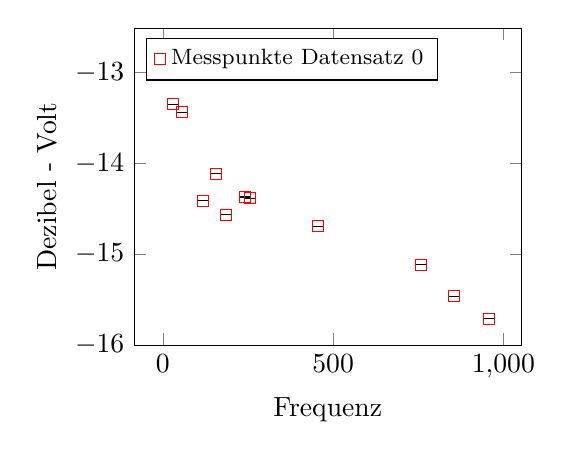
\begin{tikzpicture}
		\pgfplotsset{width=6.5cm,compat=1.3,legend style={font=\footnotesize}}
		\begin{axis}[xlabel={Frequenz},ylabel={Dezibel - Volt},legend cell align=left,legend pos=north west]
		
\addplot+[only marks,color=red,mark=square,error bars/.cd,x dir=both,x explicit,y dir=both,y explicit,error bar style={color=black}] table[x=X,y=Y,x error=xerror,y error=yerror,row sep=\\]{
			X	Y	xerror	yerror	\\
			 10.253906 	 -12.80232 	 0 	 0 	\\
			 30.761719 	 -13.347933 	 0 	 0 	\\
			 57.128906 	 -13.436821 	 0 	 0 	\\
			 118.652344 	 -14.413613 	 0 	 0 	\\
			 156.738281 	 -14.114061 	 0 	 0 	\\
			 184.570312 	 -14.565412 	 0 	 0 	\\
			 241.699219 	 -14.37053 	 0 	 0 	\\
			 254.882812 	 -14.385941 	 0 	 0 	\\
			 455.566406 	 -14.692671 	 0 	 0 	\\
			 757.324219 	 -15.117664 	 0 	 0 	\\
			 855.46875 	 -15.462831 	 0 	 0 	\\
			 958.007812 	 -15.711401 	 0 	 0 	\\
		};
		\addlegendentry{Messpunkte Datensatz 0}

		\end{axis}
		\end{tikzpicture}
	\caption{Umgebung}
	\label{fig:Umgebungsmessung}
\end{figure}

        %% \begin{figure}[H]

	\centering
	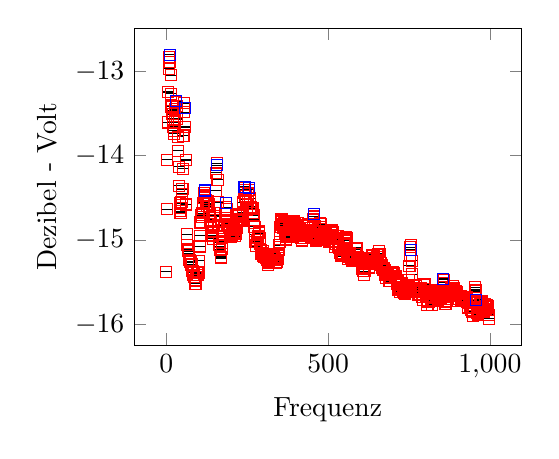
\begin{tikzpicture}
		\pgfplotsset{width=6.5cm,compat=1.3,legend style={font=\footnotesize}}
		\begin{axis}[xlabel={Frequenz},ylabel={Dezibel - Volt},legend cell align=left,legend pos=north west]
		
\addplot+[only marks,color=red,mark=square,error bars/.cd,x dir=both,x explicit,y dir=both,y explicit,error bar style={color=black}] table[x=X,y=Y,x error=xerror,y error=yerror,row sep=\\]{
			X	Y	xerror	yerror	\\
			 0.0 	 -15.377863 	 0 	 0 	\\
			 1.464844 	 -14.634824 	 0 	 0 	\\
			 2.929687 	 -14.048924 	 0 	 0 	\\
			 4.394531 	 -13.606714 	 0 	 0 	\\
			 5.859375 	 -13.245078 	 0 	 0 	\\
			 7.324219 	 -12.971722 	 0 	 0 	\\
			 8.789062 	 -12.828342 	 0 	 0 	\\
			 10.253906 	 -12.80232 	 0 	 0 	\\
			 11.71875 	 -12.891995 	 0 	 0 	\\
			 13.183594 	 -13.047378 	 0 	 0 	\\
			 14.648437 	 -13.266726 	 0 	 0 	\\
			 16.113281 	 -13.417296 	 0 	 0 	\\
			 17.578125 	 -13.467953 	 0 	 0 	\\
			 19.042969 	 -13.510851 	 0 	 0 	\\
			 20.507812 	 -13.562329 	 0 	 0 	\\
			 21.972656 	 -13.65778 	 0 	 0 	\\
			 23.4375 	 -13.742413 	 0 	 0 	\\
			 24.902344 	 -13.70612 	 0 	 0 	\\
			 26.367187 	 -13.603597 	 0 	 0 	\\
			 27.832031 	 -13.452496 	 0 	 0 	\\
			 29.296875 	 -13.360224 	 0 	 0 	\\
			 30.761719 	 -13.347933 	 0 	 0 	\\
			 32.226562 	 -13.416004 	 0 	 0 	\\
			 33.691406 	 -13.565305 	 0 	 0 	\\
			 35.15625 	 -13.777465 	 0 	 0 	\\
			 36.621094 	 -13.942297 	 0 	 0 	\\
			 38.085937 	 -14.13413 	 0 	 0 	\\
			 39.550781 	 -14.355808 	 0 	 0 	\\
			 41.015625 	 -14.567138 	 0 	 0 	\\
			 42.480469 	 -14.661787 	 0 	 0 	\\
			 43.945312 	 -14.676044 	 0 	 0 	\\
			 45.410156 	 -14.624667 	 0 	 0 	\\
			 46.875 	 -14.554264 	 0 	 0 	\\
			 48.339844 	 -14.454346 	 0 	 0 	\\
			 49.804687 	 -14.396066 	 0 	 0 	\\
			 51.269531 	 -14.157371 	 0 	 0 	\\
			 52.734375 	 -13.76188 	 0 	 0 	\\
			 54.199219 	 -13.486916 	 0 	 0 	\\
			 55.664062 	 -13.378995 	 0 	 0 	\\
			 57.128906 	 -13.436821 	 0 	 0 	\\
			 58.59375 	 -13.660917 	 0 	 0 	\\
			 60.058594 	 -14.051488 	 0 	 0 	\\
			 61.523437 	 -14.579972 	 0 	 0 	\\
			 62.988281 	 -14.932836 	 0 	 0 	\\
			 64.453125 	 -15.057708 	 0 	 0 	\\
			 65.917969 	 -15.10667 	 0 	 0 	\\
			 67.382812 	 -15.131666 	 0 	 0 	\\
			 68.847656 	 -15.120015 	 0 	 0 	\\
			 70.3125 	 -15.166563 	 0 	 0 	\\
			 71.777344 	 -15.234852 	 0 	 0 	\\
			 73.242187 	 -15.257725 	 0 	 0 	\\
			 74.707031 	 -15.258081 	 0 	 0 	\\
			 76.171875 	 -15.262162 	 0 	 0 	\\
			 77.636719 	 -15.292419 	 0 	 0 	\\
			 79.101562 	 -15.302074 	 0 	 0 	\\
			 80.566406 	 -15.371643 	 0 	 0 	\\
			 82.03125 	 -15.414623 	 0 	 0 	\\
			 83.496094 	 -15.384488 	 0 	 0 	\\
			 84.960937 	 -15.38654 	 0 	 0 	\\
			 86.425781 	 -15.435651 	 0 	 0 	\\
			 87.890625 	 -15.480934 	 0 	 0 	\\
			 89.355469 	 -15.519261 	 0 	 0 	\\
			 90.820312 	 -15.520492 	 0 	 0 	\\
			 92.285156 	 -15.435193 	 0 	 0 	\\
			 93.75 	 -15.419489 	 0 	 0 	\\
			 95.214844 	 -15.394684 	 0 	 0 	\\
			 96.679687 	 -15.392082 	 0 	 0 	\\
			 98.144531 	 -15.417509 	 0 	 0 	\\
			 99.609375 	 -15.390234 	 0 	 0 	\\
			 101.074219 	 -15.246798 	 0 	 0 	\\
			 102.539062 	 -15.077027 	 0 	 0 	\\
			 104.003906 	 -14.951796 	 0 	 0 	\\
			 105.46875 	 -14.793155 	 0 	 0 	\\
			 106.933594 	 -14.725076 	 0 	 0 	\\
			 108.398437 	 -14.70885 	 0 	 0 	\\
			 109.863281 	 -14.729992 	 0 	 0 	\\
			 111.328125 	 -14.683022 	 0 	 0 	\\
			 112.792969 	 -14.633574 	 0 	 0 	\\
			 114.257812 	 -14.559146 	 0 	 0 	\\
			 115.722656 	 -14.497235 	 0 	 0 	\\
			 117.1875 	 -14.442762 	 0 	 0 	\\
			 118.652344 	 -14.413613 	 0 	 0 	\\
			 120.117187 	 -14.473501 	 0 	 0 	\\
			 121.582031 	 -14.529763 	 0 	 0 	\\
			 123.046875 	 -14.572319 	 0 	 0 	\\
			 124.511719 	 -14.599137 	 0 	 0 	\\
			 125.976562 	 -14.57376 	 0 	 0 	\\
			 127.441406 	 -14.5452 	 0 	 0 	\\
			 128.90625 	 -14.577725 	 0 	 0 	\\
			 130.371094 	 -14.570568 	 0 	 0 	\\
			 131.835937 	 -14.606959 	 0 	 0 	\\
			 133.300781 	 -14.677834 	 0 	 0 	\\
			 134.765625 	 -14.72607 	 0 	 0 	\\
			 136.230469 	 -14.783752 	 0 	 0 	\\
			 137.695312 	 -14.845978 	 0 	 0 	\\
			 139.160156 	 -14.890022 	 0 	 0 	\\
			 140.625 	 -14.942508 	 0 	 0 	\\
			 142.089844 	 -14.958278 	 0 	 0 	\\
			 143.554687 	 -14.984087 	 0 	 0 	\\
			 145.019531 	 -14.907987 	 0 	 0 	\\
			 146.484375 	 -14.833804 	 0 	 0 	\\
			 147.949219 	 -14.760233 	 0 	 0 	\\
			 149.414062 	 -14.716789 	 0 	 0 	\\
			 150.878906 	 -14.612332 	 0 	 0 	\\
			 152.34375 	 -14.415131 	 0 	 0 	\\
			 153.808594 	 -14.203882 	 0 	 0 	\\
			 155.273437 	 -14.090973 	 0 	 0 	\\
			 156.738281 	 -14.114061 	 0 	 0 	\\
			 158.203125 	 -14.28813 	 0 	 0 	\\
			 159.667969 	 -14.549723 	 0 	 0 	\\
			 161.132812 	 -14.826476 	 0 	 0 	\\
			 162.597656 	 -15.024029 	 0 	 0 	\\
			 164.0625 	 -15.059548 	 0 	 0 	\\
			 165.527344 	 -15.076732 	 0 	 0 	\\
			 166.992187 	 -15.118956 	 0 	 0 	\\
			 168.457031 	 -15.214337 	 0 	 0 	\\
			 169.921875 	 -15.197879 	 0 	 0 	\\
			 171.386719 	 -15.102572 	 0 	 0 	\\
			 172.851562 	 -15.033952 	 0 	 0 	\\
			 174.316406 	 -14.968841 	 0 	 0 	\\
			 175.78125 	 -14.886593 	 0 	 0 	\\
			 177.246094 	 -14.857826 	 0 	 0 	\\
			 178.710937 	 -14.834681 	 0 	 0 	\\
			 180.175781 	 -14.781653 	 0 	 0 	\\
			 181.640625 	 -14.697632 	 0 	 0 	\\
			 183.105469 	 -14.612491 	 0 	 0 	\\
			 184.570312 	 -14.565412 	 0 	 0 	\\
			 186.035156 	 -14.630101 	 0 	 0 	\\
			 187.5 	 -14.763068 	 0 	 0 	\\
			 188.964844 	 -14.81181 	 0 	 0 	\\
			 190.429687 	 -14.809167 	 0 	 0 	\\
			 191.894531 	 -14.820498 	 0 	 0 	\\
			 193.359375 	 -14.83837 	 0 	 0 	\\
			 194.824219 	 -14.842676 	 0 	 0 	\\
			 196.289062 	 -14.914527 	 0 	 0 	\\
			 197.753906 	 -14.937226 	 0 	 0 	\\
			 199.21875 	 -14.963659 	 0 	 0 	\\
			 200.683594 	 -14.964335 	 0 	 0 	\\
			 202.148437 	 -14.949748 	 0 	 0 	\\
			 203.613281 	 -14.918795 	 0 	 0 	\\
			 205.078125 	 -14.910389 	 0 	 0 	\\
			 206.542969 	 -14.885805 	 0 	 0 	\\
			 208.007812 	 -14.866659 	 0 	 0 	\\
			 209.472656 	 -14.877181 	 0 	 0 	\\
			 210.9375 	 -14.919722 	 0 	 0 	\\
			 212.402344 	 -14.957385 	 0 	 0 	\\
			 213.867187 	 -14.929474 	 0 	 0 	\\
			 215.332031 	 -14.902048 	 0 	 0 	\\
			 216.796875 	 -14.855239 	 0 	 0 	\\
			 218.261719 	 -14.814927 	 0 	 0 	\\
			 219.726562 	 -14.754177 	 0 	 0 	\\
			 221.191406 	 -14.698331 	 0 	 0 	\\
			 222.65625 	 -14.7121 	 0 	 0 	\\
			 224.121094 	 -14.720584 	 0 	 0 	\\
			 225.585937 	 -14.752912 	 0 	 0 	\\
			 227.050781 	 -14.754292 	 0 	 0 	\\
			 228.515625 	 -14.7607 	 0 	 0 	\\
			 229.980469 	 -14.754367 	 0 	 0 	\\
			 231.445312 	 -14.766731 	 0 	 0 	\\
			 232.910156 	 -14.774063 	 0 	 0 	\\
			 234.375 	 -14.75994 	 0 	 0 	\\
			 235.839844 	 -14.672699 	 0 	 0 	\\
			 237.304687 	 -14.553177 	 0 	 0 	\\
			 238.769531 	 -14.442574 	 0 	 0 	\\
			 240.234375 	 -14.380149 	 0 	 0 	\\
			 241.699219 	 -14.37053 	 0 	 0 	\\
			 243.164062 	 -14.405877 	 0 	 0 	\\
			 244.628906 	 -14.478126 	 0 	 0 	\\
			 246.09375 	 -14.525214 	 0 	 0 	\\
			 247.558594 	 -14.571617 	 0 	 0 	\\
			 249.023437 	 -14.640223 	 0 	 0 	\\
			 250.488281 	 -14.62722 	 0 	 0 	\\
			 251.953125 	 -14.545152 	 0 	 0 	\\
			 253.417969 	 -14.450371 	 0 	 0 	\\
			 254.882812 	 -14.385941 	 0 	 0 	\\
			 256.347656 	 -14.403229 	 0 	 0 	\\
			 257.8125 	 -14.507634 	 0 	 0 	\\
			 259.277344 	 -14.623046 	 0 	 0 	\\
			 260.742187 	 -14.619449 	 0 	 0 	\\
			 262.207031 	 -14.607496 	 0 	 0 	\\
			 263.671875 	 -14.6373 	 0 	 0 	\\
			 265.136719 	 -14.621309 	 0 	 0 	\\
			 266.601562 	 -14.623232 	 0 	 0 	\\
			 268.066406 	 -14.675993 	 0 	 0 	\\
			 269.53125 	 -14.705281 	 0 	 0 	\\
			 270.996094 	 -14.7643 	 0 	 0 	\\
			 272.460937 	 -14.844184 	 0 	 0 	\\
			 273.925781 	 -14.933865 	 0 	 0 	\\
			 275.390625 	 -15.023675 	 0 	 0 	\\
			 276.855469 	 -15.074193 	 0 	 0 	\\
			 278.320312 	 -15.070534 	 0 	 0 	\\
			 279.785156 	 -15.020149 	 0 	 0 	\\
			 281.25 	 -14.997145 	 0 	 0 	\\
			 282.714844 	 -14.974335 	 0 	 0 	\\
			 284.179687 	 -14.95966 	 0 	 0 	\\
			 285.644531 	 -14.900165 	 0 	 0 	\\
			 287.109375 	 -14.919175 	 0 	 0 	\\
			 288.574219 	 -14.978309 	 0 	 0 	\\
			 290.039062 	 -15.051671 	 0 	 0 	\\
			 291.503906 	 -15.121433 	 0 	 0 	\\
			 292.96875 	 -15.166601 	 0 	 0 	\\
			 294.433594 	 -15.162406 	 0 	 0 	\\
			 295.898437 	 -15.158841 	 0 	 0 	\\
			 297.363281 	 -15.136656 	 0 	 0 	\\
			 298.828125 	 -15.155136 	 0 	 0 	\\
			 300.292969 	 -15.186434 	 0 	 0 	\\
			 301.757812 	 -15.204195 	 0 	 0 	\\
			 303.222656 	 -15.177276 	 0 	 0 	\\
			 304.6875 	 -15.183911 	 0 	 0 	\\
			 306.152344 	 -15.169498 	 0 	 0 	\\
			 307.617187 	 -15.183561 	 0 	 0 	\\
			 309.082031 	 -15.208333 	 0 	 0 	\\
			 310.546875 	 -15.236216 	 0 	 0 	\\
			 312.011719 	 -15.223957 	 0 	 0 	\\
			 313.476562 	 -15.265625 	 0 	 0 	\\
			 314.941406 	 -15.293078 	 0 	 0 	\\
			 316.40625 	 -15.269928 	 0 	 0 	\\
			 317.871094 	 -15.246589 	 0 	 0 	\\
			 319.335937 	 -15.235773 	 0 	 0 	\\
			 320.800781 	 -15.236421 	 0 	 0 	\\
			 322.265625 	 -15.202186 	 0 	 0 	\\
			 323.730469 	 -15.174848 	 0 	 0 	\\
			 325.195312 	 -15.166102 	 0 	 0 	\\
			 326.660156 	 -15.188197 	 0 	 0 	\\
			 328.125 	 -15.181395 	 0 	 0 	\\
			 329.589844 	 -15.162683 	 0 	 0 	\\
			 331.054687 	 -15.166449 	 0 	 0 	\\
			 332.519531 	 -15.196976 	 0 	 0 	\\
			 333.984375 	 -15.217628 	 0 	 0 	\\
			 335.449219 	 -15.211973 	 0 	 0 	\\
			 336.914062 	 -15.242704 	 0 	 0 	\\
			 338.378906 	 -15.267842 	 0 	 0 	\\
			 339.84375 	 -15.270764 	 0 	 0 	\\
			 341.308594 	 -15.259543 	 0 	 0 	\\
			 342.773437 	 -15.233829 	 0 	 0 	\\
			 344.238281 	 -15.219391 	 0 	 0 	\\
			 345.703125 	 -15.173472 	 0 	 0 	\\
			 347.167969 	 -15.116821 	 0 	 0 	\\
			 348.632812 	 -15.060204 	 0 	 0 	\\
			 350.097656 	 -15.020687 	 0 	 0 	\\
			 351.5625 	 -14.95811 	 0 	 0 	\\
			 353.027344 	 -14.843255 	 0 	 0 	\\
			 354.492187 	 -14.770459 	 0 	 0 	\\
			 355.957031 	 -14.749877 	 0 	 0 	\\
			 357.421875 	 -14.790935 	 0 	 0 	\\
			 358.886719 	 -14.815091 	 0 	 0 	\\
			 360.351562 	 -14.829277 	 0 	 0 	\\
			 361.816406 	 -14.859088 	 0 	 0 	\\
			 363.28125 	 -14.840884 	 0 	 0 	\\
			 364.746094 	 -14.800479 	 0 	 0 	\\
			 366.210937 	 -14.83119 	 0 	 0 	\\
			 367.675781 	 -14.922398 	 0 	 0 	\\
			 369.140625 	 -14.984439 	 0 	 0 	\\
			 370.605469 	 -15.002639 	 0 	 0 	\\
			 372.070312 	 -14.9656 	 0 	 0 	\\
			 373.535156 	 -14.9294 	 0 	 0 	\\
			 375.0 	 -14.915619 	 0 	 0 	\\
			 376.464844 	 -14.935517 	 0 	 0 	\\
			 377.929687 	 -14.91687 	 0 	 0 	\\
			 379.394531 	 -14.875338 	 0 	 0 	\\
			 380.859375 	 -14.886914 	 0 	 0 	\\
			 382.324219 	 -14.926704 	 0 	 0 	\\
			 383.789062 	 -14.958619 	 0 	 0 	\\
			 385.253906 	 -14.929833 	 0 	 0 	\\
			 386.71875 	 -14.858562 	 0 	 0 	\\
			 388.183594 	 -14.86051 	 0 	 0 	\\
			 389.648437 	 -14.830076 	 0 	 0 	\\
			 391.113281 	 -14.821938 	 0 	 0 	\\
			 392.578125 	 -14.818603 	 0 	 0 	\\
			 394.042969 	 -14.787719 	 0 	 0 	\\
			 395.507812 	 -14.77604 	 0 	 0 	\\
			 396.972656 	 -14.806179 	 0 	 0 	\\
			 398.4375 	 -14.859224 	 0 	 0 	\\
			 399.902344 	 -14.943791 	 0 	 0 	\\
			 401.367187 	 -14.912992 	 0 	 0 	\\
			 402.832031 	 -14.871232 	 0 	 0 	\\
			 404.296875 	 -14.852966 	 0 	 0 	\\
			 405.761719 	 -14.800711 	 0 	 0 	\\
			 407.226562 	 -14.830097 	 0 	 0 	\\
			 408.691406 	 -14.862748 	 0 	 0 	\\
			 410.15625 	 -14.903424 	 0 	 0 	\\
			 411.621094 	 -14.881023 	 0 	 0 	\\
			 413.085937 	 -14.860914 	 0 	 0 	\\
			 414.550781 	 -14.886766 	 0 	 0 	\\
			 416.015625 	 -14.925458 	 0 	 0 	\\
			 417.480469 	 -14.982026 	 0 	 0 	\\
			 418.945312 	 -14.996119 	 0 	 0 	\\
			 420.410156 	 -15.012344 	 0 	 0 	\\
			 421.875 	 -14.978925 	 0 	 0 	\\
			 423.339844 	 -14.979966 	 0 	 0 	\\
			 424.804687 	 -14.976032 	 0 	 0 	\\
			 426.269531 	 -14.953691 	 0 	 0 	\\
			 427.734375 	 -14.937518 	 0 	 0 	\\
			 429.199219 	 -14.914414 	 0 	 0 	\\
			 430.664062 	 -14.898355 	 0 	 0 	\\
			 432.128906 	 -14.90933 	 0 	 0 	\\
			 433.59375 	 -14.904637 	 0 	 0 	\\
			 435.058594 	 -14.859341 	 0 	 0 	\\
			 436.523437 	 -14.821858 	 0 	 0 	\\
			 437.988281 	 -14.816956 	 0 	 0 	\\
			 439.453125 	 -14.840019 	 0 	 0 	\\
			 440.917969 	 -14.905879 	 0 	 0 	\\
			 442.382812 	 -14.931551 	 0 	 0 	\\
			 443.847656 	 -14.948507 	 0 	 0 	\\
			 445.3125 	 -14.957315 	 0 	 0 	\\
			 446.777344 	 -14.962708 	 0 	 0 	\\
			 448.242187 	 -14.959279 	 0 	 0 	\\
			 449.707031 	 -14.976118 	 0 	 0 	\\
			 451.171875 	 -14.958943 	 0 	 0 	\\
			 452.636719 	 -14.887534 	 0 	 0 	\\
			 454.101562 	 -14.757729 	 0 	 0 	\\
			 455.566406 	 -14.692671 	 0 	 0 	\\
			 457.03125 	 -14.722008 	 0 	 0 	\\
			 458.496094 	 -14.836651 	 0 	 0 	\\
			 459.960937 	 -14.94227 	 0 	 0 	\\
			 461.425781 	 -15.008921 	 0 	 0 	\\
			 462.890625 	 -14.996549 	 0 	 0 	\\
			 464.355469 	 -14.985025 	 0 	 0 	\\
			 465.820312 	 -14.988841 	 0 	 0 	\\
			 467.285156 	 -14.959832 	 0 	 0 	\\
			 468.75 	 -14.963813 	 0 	 0 	\\
			 470.214844 	 -14.904158 	 0 	 0 	\\
			 471.679687 	 -14.899158 	 0 	 0 	\\
			 473.144531 	 -14.90094 	 0 	 0 	\\
			 474.609375 	 -14.848906 	 0 	 0 	\\
			 476.074219 	 -14.804283 	 0 	 0 	\\
			 477.539062 	 -14.812484 	 0 	 0 	\\
			 479.003906 	 -14.873761 	 0 	 0 	\\
			 480.46875 	 -14.889497 	 0 	 0 	\\
			 481.933594 	 -14.94114 	 0 	 0 	\\
			 483.398437 	 -14.959876 	 0 	 0 	\\
			 484.863281 	 -14.981784 	 0 	 0 	\\
			 486.328125 	 -15.002628 	 0 	 0 	\\
			 487.792969 	 -14.986382 	 0 	 0 	\\
			 489.257812 	 -14.958831 	 0 	 0 	\\
			 490.722656 	 -14.924504 	 0 	 0 	\\
			 492.1875 	 -14.919779 	 0 	 0 	\\
			 493.652344 	 -14.916625 	 0 	 0 	\\
			 495.117187 	 -14.949242 	 0 	 0 	\\
			 496.582031 	 -14.962884 	 0 	 0 	\\
			 498.046875 	 -14.955165 	 0 	 0 	\\
			 499.511719 	 -14.956127 	 0 	 0 	\\
			 500.976562 	 -14.98079 	 0 	 0 	\\
			 502.441406 	 -15.013497 	 0 	 0 	\\
			 503.90625 	 -15.017682 	 0 	 0 	\\
			 505.371094 	 -14.968866 	 0 	 0 	\\
			 506.835937 	 -14.974244 	 0 	 0 	\\
			 508.300781 	 -14.9413 	 0 	 0 	\\
			 509.765625 	 -14.899098 	 0 	 0 	\\
			 511.230469 	 -14.881912 	 0 	 0 	\\
			 512.695312 	 -14.900233 	 0 	 0 	\\
			 514.160156 	 -14.912839 	 0 	 0 	\\
			 515.625 	 -14.946873 	 0 	 0 	\\
			 517.089844 	 -14.979354 	 0 	 0 	\\
			 518.554687 	 -15.00894 	 0 	 0 	\\
			 520.019531 	 -15.051378 	 0 	 0 	\\
			 521.484375 	 -15.07899 	 0 	 0 	\\
			 522.949219 	 -15.042952 	 0 	 0 	\\
			 524.414062 	 -15.007503 	 0 	 0 	\\
			 525.878906 	 -14.988524 	 0 	 0 	\\
			 527.34375 	 -14.957197 	 0 	 0 	\\
			 528.808594 	 -14.957643 	 0 	 0 	\\
			 530.273437 	 -14.989294 	 0 	 0 	\\
			 531.738281 	 -15.07429 	 0 	 0 	\\
			 533.203125 	 -15.091988 	 0 	 0 	\\
			 534.667969 	 -15.084726 	 0 	 0 	\\
			 536.132812 	 -15.118594 	 0 	 0 	\\
			 537.597656 	 -15.153552 	 0 	 0 	\\
			 539.0625 	 -15.189469 	 0 	 0 	\\
			 540.527344 	 -15.190528 	 0 	 0 	\\
			 541.992187 	 -15.173378 	 0 	 0 	\\
			 543.457031 	 -15.178132 	 0 	 0 	\\
			 544.921875 	 -15.165173 	 0 	 0 	\\
			 546.386719 	 -15.114103 	 0 	 0 	\\
			 547.851562 	 -15.103409 	 0 	 0 	\\
			 549.316406 	 -15.065115 	 0 	 0 	\\
			 550.78125 	 -15.039258 	 0 	 0 	\\
			 552.246094 	 -15.00732 	 0 	 0 	\\
			 553.710937 	 -14.994949 	 0 	 0 	\\
			 555.175781 	 -14.970948 	 0 	 0 	\\
			 556.640625 	 -14.973621 	 0 	 0 	\\
			 558.105469 	 -15.052147 	 0 	 0 	\\
			 559.570312 	 -15.154666 	 0 	 0 	\\
			 561.035156 	 -15.223556 	 0 	 0 	\\
			 562.5 	 -15.205299 	 0 	 0 	\\
			 563.964844 	 -15.185758 	 0 	 0 	\\
			 565.429687 	 -15.153672 	 0 	 0 	\\
			 566.894531 	 -15.161342 	 0 	 0 	\\
			 568.359375 	 -15.174439 	 0 	 0 	\\
			 569.824219 	 -15.223043 	 0 	 0 	\\
			 571.289062 	 -15.226492 	 0 	 0 	\\
			 572.753906 	 -15.244243 	 0 	 0 	\\
			 574.21875 	 -15.246913 	 0 	 0 	\\
			 575.683594 	 -15.249243 	 0 	 0 	\\
			 577.148437 	 -15.218895 	 0 	 0 	\\
			 578.613281 	 -15.21606 	 0 	 0 	\\
			 580.078125 	 -15.209814 	 0 	 0 	\\
			 581.542969 	 -15.22923 	 0 	 0 	\\
			 583.007812 	 -15.202847 	 0 	 0 	\\
			 584.472656 	 -15.168714 	 0 	 0 	\\
			 585.9375 	 -15.112795 	 0 	 0 	\\
			 587.402344 	 -15.093079 	 0 	 0 	\\
			 588.867187 	 -15.099123 	 0 	 0 	\\
			 590.332031 	 -15.169947 	 0 	 0 	\\
			 591.796875 	 -15.199622 	 0 	 0 	\\
			 593.261719 	 -15.229956 	 0 	 0 	\\
			 594.726562 	 -15.235358 	 0 	 0 	\\
			 596.191406 	 -15.214944 	 0 	 0 	\\
			 597.65625 	 -15.24572 	 0 	 0 	\\
			 599.121094 	 -15.22883 	 0 	 0 	\\
			 600.585937 	 -15.231044 	 0 	 0 	\\
			 602.050781 	 -15.238379 	 0 	 0 	\\
			 603.515625 	 -15.2394 	 0 	 0 	\\
			 604.980469 	 -15.283166 	 0 	 0 	\\
			 606.445312 	 -15.340901 	 0 	 0 	\\
			 607.910156 	 -15.335839 	 0 	 0 	\\
			 609.375 	 -15.37254 	 0 	 0 	\\
			 610.839844 	 -15.413192 	 0 	 0 	\\
			 612.304687 	 -15.373417 	 0 	 0 	\\
			 613.769531 	 -15.323639 	 0 	 0 	\\
			 615.234375 	 -15.275425 	 0 	 0 	\\
			 616.699219 	 -15.263429 	 0 	 0 	\\
			 618.164062 	 -15.250132 	 0 	 0 	\\
			 619.628906 	 -15.267253 	 0 	 0 	\\
			 621.09375 	 -15.26846 	 0 	 0 	\\
			 622.558594 	 -15.248096 	 0 	 0 	\\
			 624.023437 	 -15.281112 	 0 	 0 	\\
			 625.488281 	 -15.332221 	 0 	 0 	\\
			 626.953125 	 -15.325418 	 0 	 0 	\\
			 628.417969 	 -15.289986 	 0 	 0 	\\
			 629.882812 	 -15.286293 	 0 	 0 	\\
			 631.347656 	 -15.279109 	 0 	 0 	\\
			 632.8125 	 -15.259318 	 0 	 0 	\\
			 634.277344 	 -15.219471 	 0 	 0 	\\
			 635.742187 	 -15.190152 	 0 	 0 	\\
			 637.207031 	 -15.17394 	 0 	 0 	\\
			 638.671875 	 -15.185223 	 0 	 0 	\\
			 640.136719 	 -15.193695 	 0 	 0 	\\
			 641.601562 	 -15.229764 	 0 	 0 	\\
			 643.066406 	 -15.250337 	 0 	 0 	\\
			 644.53125 	 -15.272403 	 0 	 0 	\\
			 645.996094 	 -15.274543 	 0 	 0 	\\
			 647.460937 	 -15.258597 	 0 	 0 	\\
			 648.925781 	 -15.25687 	 0 	 0 	\\
			 650.390625 	 -15.235247 	 0 	 0 	\\
			 651.855469 	 -15.174024 	 0 	 0 	\\
			 653.320312 	 -15.177223 	 0 	 0 	\\
			 654.785156 	 -15.166174 	 0 	 0 	\\
			 656.25 	 -15.136456 	 0 	 0 	\\
			 657.714844 	 -15.134069 	 0 	 0 	\\
			 659.179687 	 -15.172512 	 0 	 0 	\\
			 660.644531 	 -15.200877 	 0 	 0 	\\
			 662.109375 	 -15.271783 	 0 	 0 	\\
			 663.574219 	 -15.292622 	 0 	 0 	\\
			 665.039062 	 -15.30175 	 0 	 0 	\\
			 666.503906 	 -15.322372 	 0 	 0 	\\
			 667.96875 	 -15.334441 	 0 	 0 	\\
			 669.433594 	 -15.342618 	 0 	 0 	\\
			 670.898437 	 -15.354524 	 0 	 0 	\\
			 672.363281 	 -15.332675 	 0 	 0 	\\
			 673.828125 	 -15.351229 	 0 	 0 	\\
			 675.292969 	 -15.355035 	 0 	 0 	\\
			 676.757812 	 -15.410555 	 0 	 0 	\\
			 678.222656 	 -15.454251 	 0 	 0 	\\
			 679.6875 	 -15.40483 	 0 	 0 	\\
			 681.152344 	 -15.387011 	 0 	 0 	\\
			 682.617187 	 -15.381831 	 0 	 0 	\\
			 684.082031 	 -15.380513 	 0 	 0 	\\
			 685.546875 	 -15.413772 	 0 	 0 	\\
			 687.011719 	 -15.445245 	 0 	 0 	\\
			 688.476562 	 -15.487407 	 0 	 0 	\\
			 689.941406 	 -15.484309 	 0 	 0 	\\
			 691.40625 	 -15.482493 	 0 	 0 	\\
			 692.871094 	 -15.439923 	 0 	 0 	\\
			 694.335937 	 -15.407051 	 0 	 0 	\\
			 695.800781 	 -15.395723 	 0 	 0 	\\
			 697.265625 	 -15.401745 	 0 	 0 	\\
			 698.730469 	 -15.391471 	 0 	 0 	\\
			 700.195312 	 -15.385299 	 0 	 0 	\\
			 701.660156 	 -15.398126 	 0 	 0 	\\
			 703.125 	 -15.406516 	 0 	 0 	\\
			 704.589844 	 -15.389331 	 0 	 0 	\\
			 706.054687 	 -15.427444 	 0 	 0 	\\
			 707.519531 	 -15.431758 	 0 	 0 	\\
			 708.984375 	 -15.425674 	 0 	 0 	\\
			 710.449219 	 -15.446452 	 0 	 0 	\\
			 711.914062 	 -15.474679 	 0 	 0 	\\
			 713.378906 	 -15.525805 	 0 	 0 	\\
			 714.84375 	 -15.589171 	 0 	 0 	\\
			 716.308594 	 -15.586641 	 0 	 0 	\\
			 717.773437 	 -15.587684 	 0 	 0 	\\
			 719.238281 	 -15.595326 	 0 	 0 	\\
			 720.703125 	 -15.593172 	 0 	 0 	\\
			 722.167969 	 -15.615338 	 0 	 0 	\\
			 723.632812 	 -15.574624 	 0 	 0 	\\
			 725.097656 	 -15.560847 	 0 	 0 	\\
			 726.5625 	 -15.50968 	 0 	 0 	\\
			 728.027344 	 -15.50755 	 0 	 0 	\\
			 729.492187 	 -15.529643 	 0 	 0 	\\
			 730.957031 	 -15.584285 	 0 	 0 	\\
			 732.421875 	 -15.61486 	 0 	 0 	\\
			 733.886719 	 -15.607152 	 0 	 0 	\\
			 735.351562 	 -15.62397 	 0 	 0 	\\
			 736.816406 	 -15.634898 	 0 	 0 	\\
			 738.28125 	 -15.635034 	 0 	 0 	\\
			 739.746094 	 -15.61694 	 0 	 0 	\\
			 741.210937 	 -15.600624 	 0 	 0 	\\
			 742.675781 	 -15.597813 	 0 	 0 	\\
			 744.140625 	 -15.580082 	 0 	 0 	\\
			 745.605469 	 -15.576345 	 0 	 0 	\\
			 747.070312 	 -15.593973 	 0 	 0 	\\
			 748.535156 	 -15.552722 	 0 	 0 	\\
			 750.0 	 -15.48038 	 0 	 0 	\\
			 751.464844 	 -15.305891 	 0 	 0 	\\
			 752.929687 	 -15.187352 	 0 	 0 	\\
			 754.394531 	 -15.086647 	 0 	 0 	\\
			 755.859375 	 -15.058162 	 0 	 0 	\\
			 757.324219 	 -15.117664 	 0 	 0 	\\
			 758.789062 	 -15.246047 	 0 	 0 	\\
			 760.253906 	 -15.409334 	 0 	 0 	\\
			 761.71875 	 -15.531305 	 0 	 0 	\\
			 763.183594 	 -15.610576 	 0 	 0 	\\
			 764.648437 	 -15.608558 	 0 	 0 	\\
			 766.113281 	 -15.611633 	 0 	 0 	\\
			 767.578125 	 -15.588454 	 0 	 0 	\\
			 769.042969 	 -15.592371 	 0 	 0 	\\
			 770.507812 	 -15.545033 	 0 	 0 	\\
			 771.972656 	 -15.570368 	 0 	 0 	\\
			 773.4375 	 -15.590781 	 0 	 0 	\\
			 774.902344 	 -15.607064 	 0 	 0 	\\
			 776.367187 	 -15.585898 	 0 	 0 	\\
			 777.832031 	 -15.577243 	 0 	 0 	\\
			 779.296875 	 -15.646981 	 0 	 0 	\\
			 780.761719 	 -15.643249 	 0 	 0 	\\
			 782.226562 	 -15.638178 	 0 	 0 	\\
			 783.691406 	 -15.638564 	 0 	 0 	\\
			 785.15625 	 -15.600507 	 0 	 0 	\\
			 786.621094 	 -15.619703 	 0 	 0 	\\
			 788.085937 	 -15.571874 	 0 	 0 	\\
			 789.550781 	 -15.611286 	 0 	 0 	\\
			 791.015625 	 -15.679298 	 0 	 0 	\\
			 792.480469 	 -15.708989 	 0 	 0 	\\
			 793.945312 	 -15.715225 	 0 	 0 	\\
			 795.410156 	 -15.608697 	 0 	 0 	\\
			 796.875 	 -15.524976 	 0 	 0 	\\
			 798.339844 	 -15.528546 	 0 	 0 	\\
			 799.804687 	 -15.58165 	 0 	 0 	\\
			 801.269531 	 -15.617491 	 0 	 0 	\\
			 802.734375 	 -15.636778 	 0 	 0 	\\
			 804.199219 	 -15.671623 	 0 	 0 	\\
			 805.664062 	 -15.730237 	 0 	 0 	\\
			 807.128906 	 -15.773552 	 0 	 0 	\\
			 808.59375 	 -15.735681 	 0 	 0 	\\
			 810.058594 	 -15.737674 	 0 	 0 	\\
			 811.523437 	 -15.668612 	 0 	 0 	\\
			 812.988281 	 -15.63689 	 0 	 0 	\\
			 814.453125 	 -15.62498 	 0 	 0 	\\
			 815.917969 	 -15.617883 	 0 	 0 	\\
			 817.382812 	 -15.666109 	 0 	 0 	\\
			 818.847656 	 -15.717725 	 0 	 0 	\\
			 820.3125 	 -15.769734 	 0 	 0 	\\
			 821.777344 	 -15.72365 	 0 	 0 	\\
			 823.242187 	 -15.688064 	 0 	 0 	\\
			 824.707031 	 -15.715984 	 0 	 0 	\\
			 826.171875 	 -15.6625 	 0 	 0 	\\
			 827.636719 	 -15.61216 	 0 	 0 	\\
			 829.101562 	 -15.623609 	 0 	 0 	\\
			 830.566406 	 -15.595214 	 0 	 0 	\\
			 832.03125 	 -15.627422 	 0 	 0 	\\
			 833.496094 	 -15.660074 	 0 	 0 	\\
			 834.960937 	 -15.659803 	 0 	 0 	\\
			 836.425781 	 -15.679097 	 0 	 0 	\\
			 837.890625 	 -15.684159 	 0 	 0 	\\
			 839.355469 	 -15.704955 	 0 	 0 	\\
			 840.820312 	 -15.718154 	 0 	 0 	\\
			 842.285156 	 -15.682697 	 0 	 0 	\\
			 843.75 	 -15.641373 	 0 	 0 	\\
			 845.214844 	 -15.62105 	 0 	 0 	\\
			 846.679687 	 -15.658638 	 0 	 0 	\\
			 848.144531 	 -15.666164 	 0 	 0 	\\
			 849.609375 	 -15.682085 	 0 	 0 	\\
			 851.074219 	 -15.664447 	 0 	 0 	\\
			 852.539062 	 -15.590643 	 0 	 0 	\\
			 854.003906 	 -15.506291 	 0 	 0 	\\
			 855.46875 	 -15.462831 	 0 	 0 	\\
			 856.933594 	 -15.474423 	 0 	 0 	\\
			 858.398437 	 -15.560124 	 0 	 0 	\\
			 859.863281 	 -15.633947 	 0 	 0 	\\
			 861.328125 	 -15.72679 	 0 	 0 	\\
			 862.792969 	 -15.760758 	 0 	 0 	\\
			 864.257812 	 -15.731995 	 0 	 0 	\\
			 865.722656 	 -15.702384 	 0 	 0 	\\
			 867.1875 	 -15.67397 	 0 	 0 	\\
			 868.652344 	 -15.662891 	 0 	 0 	\\
			 870.117187 	 -15.630239 	 0 	 0 	\\
			 871.582031 	 -15.635438 	 0 	 0 	\\
			 873.046875 	 -15.621477 	 0 	 0 	\\
			 874.511719 	 -15.60827 	 0 	 0 	\\
			 875.976562 	 -15.62759 	 0 	 0 	\\
			 877.441406 	 -15.594709 	 0 	 0 	\\
			 878.90625 	 -15.585837 	 0 	 0 	\\
			 880.371094 	 -15.570807 	 0 	 0 	\\
			 881.835937 	 -15.572389 	 0 	 0 	\\
			 883.300781 	 -15.580299 	 0 	 0 	\\
			 884.765625 	 -15.577057 	 0 	 0 	\\
			 886.230469 	 -15.550639 	 0 	 0 	\\
			 887.695312 	 -15.574831 	 0 	 0 	\\
			 889.160156 	 -15.662833 	 0 	 0 	\\
			 890.625 	 -15.649592 	 0 	 0 	\\
			 892.089844 	 -15.62271 	 0 	 0 	\\
			 893.554687 	 -15.602035 	 0 	 0 	\\
			 895.019531 	 -15.636141 	 0 	 0 	\\
			 896.484375 	 -15.626822 	 0 	 0 	\\
			 897.949219 	 -15.619872 	 0 	 0 	\\
			 899.414062 	 -15.644022 	 0 	 0 	\\
			 900.878906 	 -15.667616 	 0 	 0 	\\
			 902.34375 	 -15.723701 	 0 	 0 	\\
			 903.808594 	 -15.699232 	 0 	 0 	\\
			 905.273437 	 -15.664368 	 0 	 0 	\\
			 906.738281 	 -15.666367 	 0 	 0 	\\
			 908.203125 	 -15.666335 	 0 	 0 	\\
			 909.667969 	 -15.664598 	 0 	 0 	\\
			 911.132812 	 -15.710565 	 0 	 0 	\\
			 912.597656 	 -15.689029 	 0 	 0 	\\
			 914.0625 	 -15.715661 	 0 	 0 	\\
			 915.527344 	 -15.695117 	 0 	 0 	\\
			 916.992187 	 -15.69187 	 0 	 0 	\\
			 918.457031 	 -15.680548 	 0 	 0 	\\
			 919.921875 	 -15.686535 	 0 	 0 	\\
			 921.386719 	 -15.704471 	 0 	 0 	\\
			 922.851562 	 -15.700725 	 0 	 0 	\\
			 924.316406 	 -15.678341 	 0 	 0 	\\
			 925.78125 	 -15.681353 	 0 	 0 	\\
			 927.246094 	 -15.673534 	 0 	 0 	\\
			 928.710937 	 -15.678921 	 0 	 0 	\\
			 930.175781 	 -15.737279 	 0 	 0 	\\
			 931.640625 	 -15.809987 	 0 	 0 	\\
			 933.105469 	 -15.801069 	 0 	 0 	\\
			 934.570312 	 -15.750958 	 0 	 0 	\\
			 936.035156 	 -15.720745 	 0 	 0 	\\
			 937.5 	 -15.773855 	 0 	 0 	\\
			 938.964844 	 -15.798507 	 0 	 0 	\\
			 940.429687 	 -15.83516 	 0 	 0 	\\
			 941.894531 	 -15.810615 	 0 	 0 	\\
			 943.359375 	 -15.803824 	 0 	 0 	\\
			 944.824219 	 -15.849649 	 0 	 0 	\\
			 946.289062 	 -15.854314 	 0 	 0 	\\
			 947.753906 	 -15.900403 	 0 	 0 	\\
			 949.21875 	 -15.839508 	 0 	 0 	\\
			 950.683594 	 -15.793809 	 0 	 0 	\\
			 952.148437 	 -15.721682 	 0 	 0 	\\
			 953.613281 	 -15.607086 	 0 	 0 	\\
			 955.078125 	 -15.562192 	 0 	 0 	\\
			 956.542969 	 -15.593833 	 0 	 0 	\\
			 958.007812 	 -15.711401 	 0 	 0 	\\
			 959.472656 	 -15.791427 	 0 	 0 	\\
			 960.9375 	 -15.861916 	 0 	 0 	\\
			 962.402344 	 -15.888155 	 0 	 0 	\\
			 963.867187 	 -15.879557 	 0 	 0 	\\
			 965.332031 	 -15.85072 	 0 	 0 	\\
			 966.796875 	 -15.826943 	 0 	 0 	\\
			 968.261719 	 -15.809572 	 0 	 0 	\\
			 969.726562 	 -15.762745 	 0 	 0 	\\
			 971.191406 	 -15.739539 	 0 	 0 	\\
			 972.65625 	 -15.739934 	 0 	 0 	\\
			 974.121094 	 -15.730753 	 0 	 0 	\\
			 975.585937 	 -15.749772 	 0 	 0 	\\
			 977.050781 	 -15.812438 	 0 	 0 	\\
			 978.515625 	 -15.826443 	 0 	 0 	\\
			 979.980469 	 -15.817046 	 0 	 0 	\\
			 981.445312 	 -15.848172 	 0 	 0 	\\
			 982.910156 	 -15.855113 	 0 	 0 	\\
			 984.375 	 -15.785814 	 0 	 0 	\\
			 985.839844 	 -15.756446 	 0 	 0 	\\
			 987.304687 	 -15.786946 	 0 	 0 	\\
			 988.769531 	 -15.817096 	 0 	 0 	\\
			 990.234375 	 -15.794719 	 0 	 0 	\\
			 991.699219 	 -15.768299 	 0 	 0 	\\
			 993.164062 	 -15.787708 	 0 	 0 	\\
			 994.628906 	 -15.828947 	 0 	 0 	\\
			 996.09375 	 -15.887351 	 0 	 0 	\\
			 997.558594 	 -15.934677 	 0 	 0 	\\
		};
		% \addlegendentry{Messpunkte Datensatz 0}

\addplot+[only marks,color=blue,mark=square,error bars/.cd,x dir=both,x explicit,y dir=both,y explicit,error bar style={color=black}] table[x=X,y=Y,x error=xerror,y error=yerror,row sep=\\]{
			X	Y	xerror	yerror	\\
			 10.253906 	 -12.80232 	 0 	 0 	\\
			 30.761719 	 -13.347933 	 0 	 0 	\\
			 57.128906 	 -13.436821 	 0 	 0 	\\
			 118.652344 	 -14.413613 	 0 	 0 	\\
			 156.738281 	 -14.114061 	 0 	 0 	\\
			 184.570312 	 -14.565412 	 0 	 0 	\\
			 241.699219 	 -14.37053 	 0 	 0 	\\
			 254.882812 	 -14.385941 	 0 	 0 	\\
			 455.566406 	 -14.692671 	 0 	 0 	\\
			 757.324219 	 -15.117664 	 0 	 0 	\\
			 855.46875 	 -15.462831 	 0 	 0 	\\
			 958.007812 	 -15.711401 	 0 	 0 	\\
		};
		% \addlegendentry{Messpunkte Datensatz 1}

		\end{axis}
		\end{tikzpicture}
	\caption{Umgebung}
	\label{fig:Umgebungsmessung}
\end{figure}


        %\begin{figure}[H]

	\centering
	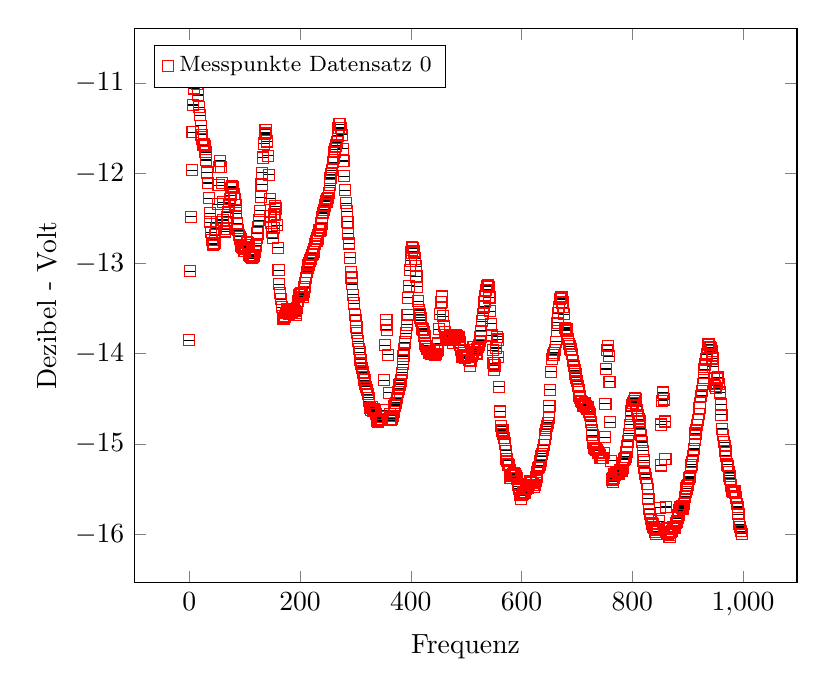
\begin{tikzpicture}
		\pgfplotsset{width=10cm,compat=1.3,legend style={font=\footnotesize}}
		\begin{axis}[xlabel={Frequenz},ylabel={Dezibel - Volt},legend cell align=left,legend pos=north west]
		
\addplot+[only marks,color=red,mark=square,error bars/.cd,x dir=both,x explicit,y dir=both,y explicit,error bar style={color=black}] table[x=X,y=Y,x error=xerror,y error=yerror,row sep=\\]{
			X	Y	xerror	yerror	\\
			 0.0 	 -13.848843 	 0 	 0 	\\
			 1.464844 	 -13.084864 	 0 	 0 	\\
			 2.929687 	 -12.482075 	 0 	 0 	\\
			 4.394531 	 -11.965661 	 0 	 0 	\\
			 5.859375 	 -11.546794 	 0 	 0 	\\
			 7.324219 	 -11.244475 	 0 	 0 	\\
			 8.789062 	 -11.060753 	 0 	 0 	\\
			 10.253906 	 -10.930851 	 0 	 0 	\\
			 11.71875 	 -10.905362 	 0 	 0 	\\
			 13.183594 	 -10.945357 	 0 	 0 	\\
			 14.648437 	 -11.015081 	 0 	 0 	\\
			 16.113281 	 -11.133686 	 0 	 0 	\\
			 17.578125 	 -11.268296 	 0 	 0 	\\
			 19.042969 	 -11.358805 	 0 	 0 	\\
			 20.507812 	 -11.472242 	 0 	 0 	\\
			 21.972656 	 -11.572217 	 0 	 0 	\\
			 23.4375 	 -11.621438 	 0 	 0 	\\
			 24.902344 	 -11.691274 	 0 	 0 	\\
			 26.367187 	 -11.680804 	 0 	 0 	\\
			 27.832031 	 -11.699508 	 0 	 0 	\\
			 29.296875 	 -11.7647 	 0 	 0 	\\
			 30.761719 	 -11.852881 	 0 	 0 	\\
			 32.226562 	 -11.99242 	 0 	 0 	\\
			 33.691406 	 -12.107867 	 0 	 0 	\\
			 35.15625 	 -12.275713 	 0 	 0 	\\
			 36.621094 	 -12.441633 	 0 	 0 	\\
			 38.085937 	 -12.54294 	 0 	 0 	\\
			 39.550781 	 -12.651932 	 0 	 0 	\\
			 41.015625 	 -12.737365 	 0 	 0 	\\
			 42.480469 	 -12.788693 	 0 	 0 	\\
			 43.945312 	 -12.777987 	 0 	 0 	\\
			 45.410156 	 -12.77724 	 0 	 0 	\\
			 46.875 	 -12.68664 	 0 	 0 	\\
			 48.339844 	 -12.616001 	 0 	 0 	\\
			 49.804687 	 -12.544291 	 0 	 0 	\\
			 51.269531 	 -12.344349 	 0 	 0 	\\
			 52.734375 	 -12.132418 	 0 	 0 	\\
			 54.199219 	 -11.929949 	 0 	 0 	\\
			 55.664062 	 -11.861673 	 0 	 0 	\\
			 57.128906 	 -11.927901 	 0 	 0 	\\
			 58.59375 	 -12.103909 	 0 	 0 	\\
			 60.058594 	 -12.32203 	 0 	 0 	\\
			 61.523437 	 -12.517847 	 0 	 0 	\\
			 62.988281 	 -12.616468 	 0 	 0 	\\
			 64.453125 	 -12.645748 	 0 	 0 	\\
			 65.917969 	 -12.61736 	 0 	 0 	\\
			 67.382812 	 -12.552704 	 0 	 0 	\\
			 68.847656 	 -12.484294 	 0 	 0 	\\
			 70.3125 	 -12.432589 	 0 	 0 	\\
			 71.777344 	 -12.339848 	 0 	 0 	\\
			 73.242187 	 -12.285835 	 0 	 0 	\\
			 74.707031 	 -12.244226 	 0 	 0 	\\
			 76.171875 	 -12.159871 	 0 	 0 	\\
			 77.636719 	 -12.146492 	 0 	 0 	\\
			 79.101562 	 -12.15427 	 0 	 0 	\\
			 80.566406 	 -12.22811 	 0 	 0 	\\
			 82.03125 	 -12.288702 	 0 	 0 	\\
			 83.496094 	 -12.357264 	 0 	 0 	\\
			 84.960937 	 -12.44275 	 0 	 0 	\\
			 86.425781 	 -12.553677 	 0 	 0 	\\
			 87.890625 	 -12.6296 	 0 	 0 	\\
			 89.355469 	 -12.688173 	 0 	 0 	\\
			 90.820312 	 -12.704946 	 0 	 0 	\\
			 92.285156 	 -12.731203 	 0 	 0 	\\
			 93.75 	 -12.801209 	 0 	 0 	\\
			 95.214844 	 -12.81376 	 0 	 0 	\\
			 96.679687 	 -12.822852 	 0 	 0 	\\
			 98.144531 	 -12.862325 	 0 	 0 	\\
			 99.609375 	 -12.835527 	 0 	 0 	\\
			 101.074219 	 -12.861899 	 0 	 0 	\\
			 102.539062 	 -12.796264 	 0 	 0 	\\
			 104.003906 	 -12.767695 	 0 	 0 	\\
			 105.46875 	 -12.776719 	 0 	 0 	\\
			 106.933594 	 -12.820479 	 0 	 0 	\\
			 108.398437 	 -12.902568 	 0 	 0 	\\
			 109.863281 	 -12.912542 	 0 	 0 	\\
			 111.328125 	 -12.925619 	 0 	 0 	\\
			 112.792969 	 -12.94205 	 0 	 0 	\\
			 114.257812 	 -12.925128 	 0 	 0 	\\
			 115.722656 	 -12.917577 	 0 	 0 	\\
			 117.1875 	 -12.910091 	 0 	 0 	\\
			 118.652344 	 -12.877029 	 0 	 0 	\\
			 120.117187 	 -12.804531 	 0 	 0 	\\
			 121.582031 	 -12.721627 	 0 	 0 	\\
			 123.046875 	 -12.667387 	 0 	 0 	\\
			 124.511719 	 -12.593013 	 0 	 0 	\\
			 125.976562 	 -12.521207 	 0 	 0 	\\
			 127.441406 	 -12.417398 	 0 	 0 	\\
			 128.90625 	 -12.265208 	 0 	 0 	\\
			 130.371094 	 -12.125359 	 0 	 0 	\\
			 131.835937 	 -11.994921 	 0 	 0 	\\
			 133.300781 	 -11.826387 	 0 	 0 	\\
			 134.765625 	 -11.671044 	 0 	 0 	\\
			 136.230469 	 -11.565237 	 0 	 0 	\\
			 137.695312 	 -11.518209 	 0 	 0 	\\
			 139.160156 	 -11.552087 	 0 	 0 	\\
			 140.625 	 -11.648033 	 0 	 0 	\\
			 142.089844 	 -11.807956 	 0 	 0 	\\
			 143.554687 	 -12.018671 	 0 	 0 	\\
			 145.019531 	 -12.281651 	 0 	 0 	\\
			 146.484375 	 -12.478611 	 0 	 0 	\\
			 147.949219 	 -12.546177 	 0 	 0 	\\
			 149.414062 	 -12.648767 	 0 	 0 	\\
			 150.878906 	 -12.717481 	 0 	 0 	\\
			 152.34375 	 -12.60883 	 0 	 0 	\\
			 153.808594 	 -12.45765 	 0 	 0 	\\
			 155.273437 	 -12.368136 	 0 	 0 	\\
			 156.738281 	 -12.391095 	 0 	 0 	\\
			 158.203125 	 -12.574885 	 0 	 0 	\\
			 159.667969 	 -12.825482 	 0 	 0 	\\
			 161.132812 	 -13.075072 	 0 	 0 	\\
			 162.597656 	 -13.229819 	 0 	 0 	\\
			 164.0625 	 -13.330846 	 0 	 0 	\\
			 165.527344 	 -13.396548 	 0 	 0 	\\
			 166.992187 	 -13.48553 	 0 	 0 	\\
			 168.457031 	 -13.585124 	 0 	 0 	\\
			 169.921875 	 -13.610015 	 0 	 0 	\\
			 171.386719 	 -13.605334 	 0 	 0 	\\
			 172.851562 	 -13.591405 	 0 	 0 	\\
			 174.316406 	 -13.544796 	 0 	 0 	\\
			 175.78125 	 -13.542664 	 0 	 0 	\\
			 177.246094 	 -13.510556 	 0 	 0 	\\
			 178.710937 	 -13.52105 	 0 	 0 	\\
			 180.175781 	 -13.553794 	 0 	 0 	\\
			 181.640625 	 -13.548846 	 0 	 0 	\\
			 183.105469 	 -13.544876 	 0 	 0 	\\
			 184.570312 	 -13.54253 	 0 	 0 	\\
			 186.035156 	 -13.513837 	 0 	 0 	\\
			 187.5 	 -13.507518 	 0 	 0 	\\
			 188.964844 	 -13.50047 	 0 	 0 	\\
			 190.429687 	 -13.527512 	 0 	 0 	\\
			 191.894531 	 -13.570786 	 0 	 0 	\\
			 193.359375 	 -13.552947 	 0 	 0 	\\
			 194.824219 	 -13.494712 	 0 	 0 	\\
			 196.289062 	 -13.41887 	 0 	 0 	\\
			 197.753906 	 -13.353909 	 0 	 0 	\\
			 199.21875 	 -13.337684 	 0 	 0 	\\
			 200.683594 	 -13.351425 	 0 	 0 	\\
			 202.148437 	 -13.330976 	 0 	 0 	\\
			 203.613281 	 -13.34627 	 0 	 0 	\\
			 205.078125 	 -13.370569 	 0 	 0 	\\
			 206.542969 	 -13.317163 	 0 	 0 	\\
			 208.007812 	 -13.262286 	 0 	 0 	\\
			 209.472656 	 -13.217603 	 0 	 0 	\\
			 210.9375 	 -13.157769 	 0 	 0 	\\
			 212.402344 	 -13.092333 	 0 	 0 	\\
			 213.867187 	 -13.048602 	 0 	 0 	\\
			 215.332031 	 -13.01314 	 0 	 0 	\\
			 216.796875 	 -12.999195 	 0 	 0 	\\
			 218.261719 	 -12.967447 	 0 	 0 	\\
			 219.726562 	 -12.943947 	 0 	 0 	\\
			 221.191406 	 -12.908824 	 0 	 0 	\\
			 222.65625 	 -12.892823 	 0 	 0 	\\
			 224.121094 	 -12.873651 	 0 	 0 	\\
			 225.585937 	 -12.845595 	 0 	 0 	\\
			 227.050781 	 -12.787115 	 0 	 0 	\\
			 228.515625 	 -12.751273 	 0 	 0 	\\
			 229.980469 	 -12.753224 	 0 	 0 	\\
			 231.445312 	 -12.723715 	 0 	 0 	\\
			 232.910156 	 -12.690077 	 0 	 0 	\\
			 234.375 	 -12.628439 	 0 	 0 	\\
			 235.839844 	 -12.634004 	 0 	 0 	\\
			 237.304687 	 -12.631191 	 0 	 0 	\\
			 238.769531 	 -12.556608 	 0 	 0 	\\
			 240.234375 	 -12.487989 	 0 	 0 	\\
			 241.699219 	 -12.44106 	 0 	 0 	\\
			 243.164062 	 -12.403562 	 0 	 0 	\\
			 244.628906 	 -12.357152 	 0 	 0 	\\
			 246.09375 	 -12.307795 	 0 	 0 	\\
			 247.558594 	 -12.317731 	 0 	 0 	\\
			 249.023437 	 -12.281264 	 0 	 0 	\\
			 250.488281 	 -12.27329 	 0 	 0 	\\
			 251.953125 	 -12.218162 	 0 	 0 	\\
			 253.417969 	 -12.134033 	 0 	 0 	\\
			 254.882812 	 -12.052472 	 0 	 0 	\\
			 256.347656 	 -12.011626 	 0 	 0 	\\
			 257.8125 	 -11.966825 	 0 	 0 	\\
			 259.277344 	 -11.878083 	 0 	 0 	\\
			 260.742187 	 -11.830478 	 0 	 0 	\\
			 262.207031 	 -11.761236 	 0 	 0 	\\
			 263.671875 	 -11.733871 	 0 	 0 	\\
			 265.136719 	 -11.693561 	 0 	 0 	\\
			 266.601562 	 -11.65706 	 0 	 0 	\\
			 268.066406 	 -11.581274 	 0 	 0 	\\
			 269.53125 	 -11.497283 	 0 	 0 	\\
			 270.996094 	 -11.455608 	 0 	 0 	\\
			 272.460937 	 -11.459285 	 0 	 0 	\\
			 273.925781 	 -11.501212 	 0 	 0 	\\
			 275.390625 	 -11.572617 	 0 	 0 	\\
			 276.855469 	 -11.727455 	 0 	 0 	\\
			 278.320312 	 -11.864044 	 0 	 0 	\\
			 279.785156 	 -12.032756 	 0 	 0 	\\
			 281.25 	 -12.188835 	 0 	 0 	\\
			 282.714844 	 -12.331757 	 0 	 0 	\\
			 284.179687 	 -12.420208 	 0 	 0 	\\
			 285.644531 	 -12.53871 	 0 	 0 	\\
			 287.109375 	 -12.671718 	 0 	 0 	\\
			 288.574219 	 -12.778358 	 0 	 0 	\\
			 290.039062 	 -12.93537 	 0 	 0 	\\
			 291.503906 	 -13.090729 	 0 	 0 	\\
			 292.96875 	 -13.155254 	 0 	 0 	\\
			 294.433594 	 -13.231764 	 0 	 0 	\\
			 295.898437 	 -13.346051 	 0 	 0 	\\
			 297.363281 	 -13.442986 	 0 	 0 	\\
			 298.828125 	 -13.570926 	 0 	 0 	\\
			 300.292969 	 -13.628228 	 0 	 0 	\\
			 301.757812 	 -13.707827 	 0 	 0 	\\
			 303.222656 	 -13.771672 	 0 	 0 	\\
			 304.6875 	 -13.86243 	 0 	 0 	\\
			 306.152344 	 -13.943918 	 0 	 0 	\\
			 307.617187 	 -13.982186 	 0 	 0 	\\
			 309.082031 	 -14.064806 	 0 	 0 	\\
			 310.546875 	 -14.108041 	 0 	 0 	\\
			 312.011719 	 -14.155785 	 0 	 0 	\\
			 313.476562 	 -14.207383 	 0 	 0 	\\
			 314.941406 	 -14.259609 	 0 	 0 	\\
			 316.40625 	 -14.295196 	 0 	 0 	\\
			 317.871094 	 -14.331971 	 0 	 0 	\\
			 319.335937 	 -14.366945 	 0 	 0 	\\
			 320.800781 	 -14.399659 	 0 	 0 	\\
			 322.265625 	 -14.448483 	 0 	 0 	\\
			 323.730469 	 -14.488628 	 0 	 0 	\\
			 325.195312 	 -14.527894 	 0 	 0 	\\
			 326.660156 	 -14.602149 	 0 	 0 	\\
			 328.125 	 -14.620625 	 0 	 0 	\\
			 329.589844 	 -14.593219 	 0 	 0 	\\
			 331.054687 	 -14.630564 	 0 	 0 	\\
			 332.519531 	 -14.630167 	 0 	 0 	\\
			 333.984375 	 -14.608939 	 0 	 0 	\\
			 335.449219 	 -14.636128 	 0 	 0 	\\
			 336.914062 	 -14.667382 	 0 	 0 	\\
			 338.378906 	 -14.725865 	 0 	 0 	\\
			 339.84375 	 -14.742405 	 0 	 0 	\\
			 341.308594 	 -14.755925 	 0 	 0 	\\
			 342.773437 	 -14.733687 	 0 	 0 	\\
			 344.238281 	 -14.720973 	 0 	 0 	\\
			 345.703125 	 -14.734243 	 0 	 0 	\\
			 347.167969 	 -14.721421 	 0 	 0 	\\
			 348.632812 	 -14.700672 	 0 	 0 	\\
			 350.097656 	 -14.624208 	 0 	 0 	\\
			 351.5625 	 -14.293939 	 0 	 0 	\\
			 353.027344 	 -13.905712 	 0 	 0 	\\
			 354.492187 	 -13.677462 	 0 	 0 	\\
			 355.957031 	 -13.621806 	 0 	 0 	\\
			 357.421875 	 -13.733462 	 0 	 0 	\\
			 358.886719 	 -14.009808 	 0 	 0 	\\
			 360.351562 	 -14.433584 	 0 	 0 	\\
			 361.816406 	 -14.665124 	 0 	 0 	\\
			 363.28125 	 -14.717876 	 0 	 0 	\\
			 364.746094 	 -14.737621 	 0 	 0 	\\
			 366.210937 	 -14.718402 	 0 	 0 	\\
			 367.675781 	 -14.686362 	 0 	 0 	\\
			 369.140625 	 -14.64979 	 0 	 0 	\\
			 370.605469 	 -14.578752 	 0 	 0 	\\
			 372.070312 	 -14.563558 	 0 	 0 	\\
			 373.535156 	 -14.541807 	 0 	 0 	\\
			 375.0 	 -14.491673 	 0 	 0 	\\
			 376.464844 	 -14.426708 	 0 	 0 	\\
			 377.929687 	 -14.385033 	 0 	 0 	\\
			 379.394531 	 -14.344742 	 0 	 0 	\\
			 380.859375 	 -14.338758 	 0 	 0 	\\
			 382.324219 	 -14.297165 	 0 	 0 	\\
			 383.789062 	 -14.21249 	 0 	 0 	\\
			 385.253906 	 -14.117258 	 0 	 0 	\\
			 386.71875 	 -14.024889 	 0 	 0 	\\
			 388.183594 	 -13.94739 	 0 	 0 	\\
			 389.648437 	 -13.874926 	 0 	 0 	\\
			 391.113281 	 -13.773478 	 0 	 0 	\\
			 392.578125 	 -13.67769 	 0 	 0 	\\
			 394.042969 	 -13.566935 	 0 	 0 	\\
			 395.507812 	 -13.380635 	 0 	 0 	\\
			 396.972656 	 -13.246249 	 0 	 0 	\\
			 398.4375 	 -13.075774 	 0 	 0 	\\
			 399.902344 	 -12.971014 	 0 	 0 	\\
			 401.367187 	 -12.878876 	 0 	 0 	\\
			 402.832031 	 -12.8139 	 0 	 0 	\\
			 404.296875 	 -12.828142 	 0 	 0 	\\
			 405.761719 	 -12.866463 	 0 	 0 	\\
			 407.226562 	 -12.945724 	 0 	 0 	\\
			 408.691406 	 -13.031688 	 0 	 0 	\\
			 410.15625 	 -13.14485 	 0 	 0 	\\
			 411.621094 	 -13.257695 	 0 	 0 	\\
			 413.085937 	 -13.418539 	 0 	 0 	\\
			 414.550781 	 -13.515303 	 0 	 0 	\\
			 416.015625 	 -13.560336 	 0 	 0 	\\
			 417.480469 	 -13.602901 	 0 	 0 	\\
			 418.945312 	 -13.633774 	 0 	 0 	\\
			 420.410156 	 -13.721082 	 0 	 0 	\\
			 421.875 	 -13.732183 	 0 	 0 	\\
			 423.339844 	 -13.758321 	 0 	 0 	\\
			 424.804687 	 -13.801134 	 0 	 0 	\\
			 426.269531 	 -13.888743 	 0 	 0 	\\
			 427.734375 	 -13.913864 	 0 	 0 	\\
			 429.199219 	 -13.943489 	 0 	 0 	\\
			 430.664062 	 -13.944173 	 0 	 0 	\\
			 432.128906 	 -13.951193 	 0 	 0 	\\
			 433.59375 	 -13.988607 	 0 	 0 	\\
			 435.058594 	 -13.984307 	 0 	 0 	\\
			 436.523437 	 -14.003439 	 0 	 0 	\\
			 437.988281 	 -14.003711 	 0 	 0 	\\
			 439.453125 	 -14.003144 	 0 	 0 	\\
			 440.917969 	 -13.999819 	 0 	 0 	\\
			 442.382812 	 -13.974069 	 0 	 0 	\\
			 443.847656 	 -14.010213 	 0 	 0 	\\
			 445.3125 	 -14.005608 	 0 	 0 	\\
			 446.777344 	 -13.972788 	 0 	 0 	\\
			 448.242187 	 -13.957638 	 0 	 0 	\\
			 449.707031 	 -13.886552 	 0 	 0 	\\
			 451.171875 	 -13.726927 	 0 	 0 	\\
			 452.636719 	 -13.564186 	 0 	 0 	\\
			 454.101562 	 -13.431608 	 0 	 0 	\\
			 455.566406 	 -13.365859 	 0 	 0 	\\
			 457.03125 	 -13.423494 	 0 	 0 	\\
			 458.496094 	 -13.582422 	 0 	 0 	\\
			 459.960937 	 -13.695712 	 0 	 0 	\\
			 461.425781 	 -13.759894 	 0 	 0 	\\
			 462.890625 	 -13.793842 	 0 	 0 	\\
			 464.355469 	 -13.827708 	 0 	 0 	\\
			 465.820312 	 -13.83685 	 0 	 0 	\\
			 467.285156 	 -13.830297 	 0 	 0 	\\
			 468.75 	 -13.81644 	 0 	 0 	\\
			 470.214844 	 -13.845641 	 0 	 0 	\\
			 471.679687 	 -13.829206 	 0 	 0 	\\
			 473.144531 	 -13.803917 	 0 	 0 	\\
			 474.609375 	 -13.849516 	 0 	 0 	\\
			 476.074219 	 -13.880946 	 0 	 0 	\\
			 477.539062 	 -13.848585 	 0 	 0 	\\
			 479.003906 	 -13.831017 	 0 	 0 	\\
			 480.46875 	 -13.805676 	 0 	 0 	\\
			 481.933594 	 -13.791267 	 0 	 0 	\\
			 483.398437 	 -13.800226 	 0 	 0 	\\
			 484.863281 	 -13.818996 	 0 	 0 	\\
			 486.328125 	 -13.818732 	 0 	 0 	\\
			 487.792969 	 -13.86874 	 0 	 0 	\\
			 489.257812 	 -13.907663 	 0 	 0 	\\
			 490.722656 	 -13.961497 	 0 	 0 	\\
			 492.1875 	 -14.02978 	 0 	 0 	\\
			 493.652344 	 -14.019824 	 0 	 0 	\\
			 495.117187 	 -14.010858 	 0 	 0 	\\
			 496.582031 	 -14.030786 	 0 	 0 	\\
			 498.046875 	 -14.049811 	 0 	 0 	\\
			 499.511719 	 -14.020986 	 0 	 0 	\\
			 500.976562 	 -14.028292 	 0 	 0 	\\
			 502.441406 	 -14.02857 	 0 	 0 	\\
			 503.90625 	 -14.038276 	 0 	 0 	\\
			 505.371094 	 -14.073226 	 0 	 0 	\\
			 506.835937 	 -14.139538 	 0 	 0 	\\
			 508.300781 	 -14.082113 	 0 	 0 	\\
			 509.765625 	 -14.022043 	 0 	 0 	\\
			 511.230469 	 -13.977014 	 0 	 0 	\\
			 512.695312 	 -13.928044 	 0 	 0 	\\
			 514.160156 	 -13.927798 	 0 	 0 	\\
			 515.625 	 -13.961398 	 0 	 0 	\\
			 517.089844 	 -13.9973 	 0 	 0 	\\
			 518.554687 	 -14.001409 	 0 	 0 	\\
			 520.019531 	 -13.952327 	 0 	 0 	\\
			 521.484375 	 -13.921497 	 0 	 0 	\\
			 522.949219 	 -13.899399 	 0 	 0 	\\
			 524.414062 	 -13.856237 	 0 	 0 	\\
			 525.878906 	 -13.811698 	 0 	 0 	\\
			 527.34375 	 -13.74543 	 0 	 0 	\\
			 528.808594 	 -13.640151 	 0 	 0 	\\
			 530.273437 	 -13.558892 	 0 	 0 	\\
			 531.738281 	 -13.476128 	 0 	 0 	\\
			 533.203125 	 -13.424129 	 0 	 0 	\\
			 534.667969 	 -13.361391 	 0 	 0 	\\
			 536.132812 	 -13.290147 	 0 	 0 	\\
			 537.597656 	 -13.249411 	 0 	 0 	\\
			 539.0625 	 -13.243973 	 0 	 0 	\\
			 540.527344 	 -13.258794 	 0 	 0 	\\
			 541.992187 	 -13.376017 	 0 	 0 	\\
			 543.457031 	 -13.53083 	 0 	 0 	\\
			 544.921875 	 -13.669553 	 0 	 0 	\\
			 546.386719 	 -13.797888 	 0 	 0 	\\
			 547.851562 	 -13.962575 	 0 	 0 	\\
			 549.316406 	 -14.103863 	 0 	 0 	\\
			 550.78125 	 -14.175672 	 0 	 0 	\\
			 552.246094 	 -14.129969 	 0 	 0 	\\
			 553.710937 	 -13.935889 	 0 	 0 	\\
			 555.175781 	 -13.812741 	 0 	 0 	\\
			 556.640625 	 -13.842486 	 0 	 0 	\\
			 558.105469 	 -14.0394 	 0 	 0 	\\
			 559.570312 	 -14.36572 	 0 	 0 	\\
			 561.035156 	 -14.639869 	 0 	 0 	\\
			 562.5 	 -14.803625 	 0 	 0 	\\
			 563.964844 	 -14.852777 	 0 	 0 	\\
			 565.429687 	 -14.841215 	 0 	 0 	\\
			 566.894531 	 -14.885598 	 0 	 0 	\\
			 568.359375 	 -14.93465 	 0 	 0 	\\
			 569.824219 	 -14.995193 	 0 	 0 	\\
			 571.289062 	 -15.075983 	 0 	 0 	\\
			 572.753906 	 -15.162594 	 0 	 0 	\\
			 574.21875 	 -15.184264 	 0 	 0 	\\
			 575.683594 	 -15.227345 	 0 	 0 	\\
			 577.148437 	 -15.232505 	 0 	 0 	\\
			 578.613281 	 -15.293614 	 0 	 0 	\\
			 580.078125 	 -15.372789 	 0 	 0 	\\
			 581.542969 	 -15.356886 	 0 	 0 	\\
			 583.007812 	 -15.342438 	 0 	 0 	\\
			 584.472656 	 -15.331652 	 0 	 0 	\\
			 585.9375 	 -15.325742 	 0 	 0 	\\
			 587.402344 	 -15.342131 	 0 	 0 	\\
			 588.867187 	 -15.331516 	 0 	 0 	\\
			 590.332031 	 -15.355327 	 0 	 0 	\\
			 591.796875 	 -15.381597 	 0 	 0 	\\
			 593.261719 	 -15.448496 	 0 	 0 	\\
			 594.726562 	 -15.472652 	 0 	 0 	\\
			 596.191406 	 -15.492994 	 0 	 0 	\\
			 597.65625 	 -15.566356 	 0 	 0 	\\
			 599.121094 	 -15.605995 	 0 	 0 	\\
			 600.585937 	 -15.568733 	 0 	 0 	\\
			 602.050781 	 -15.554772 	 0 	 0 	\\
			 603.515625 	 -15.53828 	 0 	 0 	\\
			 604.980469 	 -15.538965 	 0 	 0 	\\
			 606.445312 	 -15.536983 	 0 	 0 	\\
			 607.910156 	 -15.502813 	 0 	 0 	\\
			 609.375 	 -15.469022 	 0 	 0 	\\
			 610.839844 	 -15.483412 	 0 	 0 	\\
			 612.304687 	 -15.461215 	 0 	 0 	\\
			 613.769531 	 -15.456343 	 0 	 0 	\\
			 615.234375 	 -15.407683 	 0 	 0 	\\
			 616.699219 	 -15.420788 	 0 	 0 	\\
			 618.164062 	 -15.43605 	 0 	 0 	\\
			 619.628906 	 -15.432121 	 0 	 0 	\\
			 621.09375 	 -15.455558 	 0 	 0 	\\
			 622.558594 	 -15.478613 	 0 	 0 	\\
			 624.023437 	 -15.449878 	 0 	 0 	\\
			 625.488281 	 -15.404584 	 0 	 0 	\\
			 626.953125 	 -15.368659 	 0 	 0 	\\
			 628.417969 	 -15.307146 	 0 	 0 	\\
			 629.882812 	 -15.26498 	 0 	 0 	\\
			 631.347656 	 -15.254311 	 0 	 0 	\\
			 632.8125 	 -15.235234 	 0 	 0 	\\
			 634.277344 	 -15.186217 	 0 	 0 	\\
			 635.742187 	 -15.138761 	 0 	 0 	\\
			 637.207031 	 -15.106788 	 0 	 0 	\\
			 638.671875 	 -15.069259 	 0 	 0 	\\
			 640.136719 	 -15.015678 	 0 	 0 	\\
			 641.601562 	 -14.946323 	 0 	 0 	\\
			 643.066406 	 -14.888166 	 0 	 0 	\\
			 644.53125 	 -14.841577 	 0 	 0 	\\
			 645.996094 	 -14.80279 	 0 	 0 	\\
			 647.460937 	 -14.763057 	 0 	 0 	\\
			 648.925781 	 -14.707606 	 0 	 0 	\\
			 650.390625 	 -14.576478 	 0 	 0 	\\
			 651.855469 	 -14.399101 	 0 	 0 	\\
			 653.320312 	 -14.201233 	 0 	 0 	\\
			 654.785156 	 -14.05587 	 0 	 0 	\\
			 656.25 	 -14.01161 	 0 	 0 	\\
			 657.714844 	 -14.015326 	 0 	 0 	\\
			 659.179687 	 -13.989563 	 0 	 0 	\\
			 660.644531 	 -13.957742 	 0 	 0 	\\
			 662.109375 	 -13.86798 	 0 	 0 	\\
			 663.574219 	 -13.74568 	 0 	 0 	\\
			 665.039062 	 -13.655993 	 0 	 0 	\\
			 666.503906 	 -13.551404 	 0 	 0 	\\
			 667.96875 	 -13.482943 	 0 	 0 	\\
			 669.433594 	 -13.394012 	 0 	 0 	\\
			 670.898437 	 -13.376683 	 0 	 0 	\\
			 672.363281 	 -13.373598 	 0 	 0 	\\
			 673.828125 	 -13.432512 	 0 	 0 	\\
			 675.292969 	 -13.483224 	 0 	 0 	\\
			 676.757812 	 -13.563242 	 0 	 0 	\\
			 678.222656 	 -13.713531 	 0 	 0 	\\
			 679.6875 	 -13.731859 	 0 	 0 	\\
			 681.152344 	 -13.725105 	 0 	 0 	\\
			 682.617187 	 -13.746216 	 0 	 0 	\\
			 684.082031 	 -13.834937 	 0 	 0 	\\
			 685.546875 	 -13.892766 	 0 	 0 	\\
			 687.011719 	 -13.917761 	 0 	 0 	\\
			 688.476562 	 -13.944634 	 0 	 0 	\\
			 689.941406 	 -13.954781 	 0 	 0 	\\
			 691.40625 	 -14.00583 	 0 	 0 	\\
			 692.871094 	 -14.080033 	 0 	 0 	\\
			 694.335937 	 -14.13577 	 0 	 0 	\\
			 695.800781 	 -14.186631 	 0 	 0 	\\
			 697.265625 	 -14.221995 	 0 	 0 	\\
			 698.730469 	 -14.264764 	 0 	 0 	\\
			 700.195312 	 -14.304014 	 0 	 0 	\\
			 701.660156 	 -14.358989 	 0 	 0 	\\
			 703.125 	 -14.406108 	 0 	 0 	\\
			 704.589844 	 -14.467628 	 0 	 0 	\\
			 706.054687 	 -14.492406 	 0 	 0 	\\
			 707.519531 	 -14.52735 	 0 	 0 	\\
			 708.984375 	 -14.533796 	 0 	 0 	\\
			 710.449219 	 -14.557829 	 0 	 0 	\\
			 711.914062 	 -14.576191 	 0 	 0 	\\
			 713.378906 	 -14.564985 	 0 	 0 	\\
			 714.84375 	 -14.551908 	 0 	 0 	\\
			 716.308594 	 -14.585457 	 0 	 0 	\\
			 717.773437 	 -14.60963 	 0 	 0 	\\
			 719.238281 	 -14.594293 	 0 	 0 	\\
			 720.703125 	 -14.598125 	 0 	 0 	\\
			 722.167969 	 -14.644541 	 0 	 0 	\\
			 723.632812 	 -14.672808 	 0 	 0 	\\
			 725.097656 	 -14.752396 	 0 	 0 	\\
			 726.5625 	 -14.851145 	 0 	 0 	\\
			 728.027344 	 -14.90107 	 0 	 0 	\\
			 729.492187 	 -14.983686 	 0 	 0 	\\
			 730.957031 	 -15.045944 	 0 	 0 	\\
			 732.421875 	 -15.059546 	 0 	 0 	\\
			 733.886719 	 -15.05426 	 0 	 0 	\\
			 735.351562 	 -15.064187 	 0 	 0 	\\
			 736.816406 	 -15.066898 	 0 	 0 	\\
			 738.28125 	 -15.093438 	 0 	 0 	\\
			 739.746094 	 -15.100656 	 0 	 0 	\\
			 741.210937 	 -15.12522 	 0 	 0 	\\
			 742.675781 	 -15.158319 	 0 	 0 	\\
			 744.140625 	 -15.157933 	 0 	 0 	\\
			 745.605469 	 -15.158154 	 0 	 0 	\\
			 747.070312 	 -15.158847 	 0 	 0 	\\
			 748.535156 	 -15.099766 	 0 	 0 	\\
			 750.0 	 -14.92643 	 0 	 0 	\\
			 751.464844 	 -14.552396 	 0 	 0 	\\
			 752.929687 	 -14.1692 	 0 	 0 	\\
			 754.394531 	 -13.958285 	 0 	 0 	\\
			 755.859375 	 -13.911774 	 0 	 0 	\\
			 757.324219 	 -14.028664 	 0 	 0 	\\
			 758.789062 	 -14.312077 	 0 	 0 	\\
			 760.253906 	 -14.760731 	 0 	 0 	\\
			 761.71875 	 -15.184678 	 0 	 0 	\\
			 763.183594 	 -15.392624 	 0 	 0 	\\
			 764.648437 	 -15.418165 	 0 	 0 	\\
			 766.113281 	 -15.377866 	 0 	 0 	\\
			 767.578125 	 -15.336439 	 0 	 0 	\\
			 769.042969 	 -15.34766 	 0 	 0 	\\
			 770.507812 	 -15.309141 	 0 	 0 	\\
			 771.972656 	 -15.309903 	 0 	 0 	\\
			 773.4375 	 -15.321543 	 0 	 0 	\\
			 774.902344 	 -15.330109 	 0 	 0 	\\
			 776.367187 	 -15.306724 	 0 	 0 	\\
			 777.832031 	 -15.288806 	 0 	 0 	\\
			 779.296875 	 -15.301909 	 0 	 0 	\\
			 780.761719 	 -15.295229 	 0 	 0 	\\
			 782.226562 	 -15.27009 	 0 	 0 	\\
			 783.691406 	 -15.208692 	 0 	 0 	\\
			 785.15625 	 -15.171063 	 0 	 0 	\\
			 786.621094 	 -15.161349 	 0 	 0 	\\
			 788.085937 	 -15.1401 	 0 	 0 	\\
			 789.550781 	 -15.091379 	 0 	 0 	\\
			 791.015625 	 -15.026564 	 0 	 0 	\\
			 792.480469 	 -14.972059 	 0 	 0 	\\
			 793.945312 	 -14.887531 	 0 	 0 	\\
			 795.410156 	 -14.786565 	 0 	 0 	\\
			 796.875 	 -14.689001 	 0 	 0 	\\
			 798.339844 	 -14.635184 	 0 	 0 	\\
			 799.804687 	 -14.567341 	 0 	 0 	\\
			 801.269531 	 -14.541805 	 0 	 0 	\\
			 802.734375 	 -14.523753 	 0 	 0 	\\
			 804.199219 	 -14.48997 	 0 	 0 	\\
			 805.664062 	 -14.504683 	 0 	 0 	\\
			 807.128906 	 -14.57874 	 0 	 0 	\\
			 808.59375 	 -14.629734 	 0 	 0 	\\
			 810.058594 	 -14.684223 	 0 	 0 	\\
			 811.523437 	 -14.72411 	 0 	 0 	\\
			 812.988281 	 -14.750403 	 0 	 0 	\\
			 814.453125 	 -14.831126 	 0 	 0 	\\
			 815.917969 	 -14.904781 	 0 	 0 	\\
			 817.382812 	 -14.977625 	 0 	 0 	\\
			 818.847656 	 -15.07545 	 0 	 0 	\\
			 820.3125 	 -15.182081 	 0 	 0 	\\
			 821.777344 	 -15.261506 	 0 	 0 	\\
			 823.242187 	 -15.335604 	 0 	 0 	\\
			 824.707031 	 -15.375717 	 0 	 0 	\\
			 826.171875 	 -15.442172 	 0 	 0 	\\
			 827.636719 	 -15.500808 	 0 	 0 	\\
			 829.101562 	 -15.608633 	 0 	 0 	\\
			 830.566406 	 -15.724411 	 0 	 0 	\\
			 832.03125 	 -15.778374 	 0 	 0 	\\
			 833.496094 	 -15.832983 	 0 	 0 	\\
			 834.960937 	 -15.881127 	 0 	 0 	\\
			 836.425781 	 -15.888403 	 0 	 0 	\\
			 837.890625 	 -15.916879 	 0 	 0 	\\
			 839.355469 	 -15.93463 	 0 	 0 	\\
			 840.820312 	 -15.969865 	 0 	 0 	\\
			 842.285156 	 -15.994647 	 0 	 0 	\\
			 843.75 	 -15.943043 	 0 	 0 	\\
			 845.214844 	 -15.950734 	 0 	 0 	\\
			 846.679687 	 -15.938186 	 0 	 0 	\\
			 848.144531 	 -15.857123 	 0 	 0 	\\
			 849.609375 	 -15.706494 	 0 	 0 	\\
			 851.074219 	 -15.237861 	 0 	 0 	\\
			 852.539062 	 -14.784414 	 0 	 0 	\\
			 854.003906 	 -14.521018 	 0 	 0 	\\
			 855.46875 	 -14.430327 	 0 	 0 	\\
			 856.933594 	 -14.506615 	 0 	 0 	\\
			 858.398437 	 -14.750749 	 0 	 0 	\\
			 859.863281 	 -15.167859 	 0 	 0 	\\
			 861.328125 	 -15.698378 	 0 	 0 	\\
			 862.792969 	 -15.937158 	 0 	 0 	\\
			 864.257812 	 -15.996637 	 0 	 0 	\\
			 865.722656 	 -15.98979 	 0 	 0 	\\
			 867.1875 	 -16.026136 	 0 	 0 	\\
			 868.652344 	 -16.006728 	 0 	 0 	\\
			 870.117187 	 -15.977865 	 0 	 0 	\\
			 871.582031 	 -15.966749 	 0 	 0 	\\
			 873.046875 	 -15.923391 	 0 	 0 	\\
			 874.511719 	 -15.932359 	 0 	 0 	\\
			 875.976562 	 -15.931909 	 0 	 0 	\\
			 877.441406 	 -15.925212 	 0 	 0 	\\
			 878.90625 	 -15.876147 	 0 	 0 	\\
			 880.371094 	 -15.858563 	 0 	 0 	\\
			 881.835937 	 -15.824195 	 0 	 0 	\\
			 883.300781 	 -15.790751 	 0 	 0 	\\
			 884.765625 	 -15.73282 	 0 	 0 	\\
			 886.230469 	 -15.697337 	 0 	 0 	\\
			 887.695312 	 -15.69995 	 0 	 0 	\\
			 889.160156 	 -15.708749 	 0 	 0 	\\
			 890.625 	 -15.686311 	 0 	 0 	\\
			 892.089844 	 -15.716433 	 0 	 0 	\\
			 893.554687 	 -15.665769 	 0 	 0 	\\
			 895.019531 	 -15.583663 	 0 	 0 	\\
			 896.484375 	 -15.531006 	 0 	 0 	\\
			 897.949219 	 -15.492765 	 0 	 0 	\\
			 899.414062 	 -15.469691 	 0 	 0 	\\
			 900.878906 	 -15.453538 	 0 	 0 	\\
			 902.34375 	 -15.382501 	 0 	 0 	\\
			 903.808594 	 -15.366147 	 0 	 0 	\\
			 905.273437 	 -15.253802 	 0 	 0 	\\
			 906.738281 	 -15.228529 	 0 	 0 	\\
			 908.203125 	 -15.194991 	 0 	 0 	\\
			 909.667969 	 -15.130339 	 0 	 0 	\\
			 911.132812 	 -15.055083 	 0 	 0 	\\
			 912.597656 	 -14.951272 	 0 	 0 	\\
			 914.0625 	 -14.883529 	 0 	 0 	\\
			 915.527344 	 -14.843739 	 0 	 0 	\\
			 916.992187 	 -14.787547 	 0 	 0 	\\
			 918.457031 	 -14.732906 	 0 	 0 	\\
			 919.921875 	 -14.671104 	 0 	 0 	\\
			 921.386719 	 -14.602968 	 0 	 0 	\\
			 922.851562 	 -14.544416 	 0 	 0 	\\
			 924.316406 	 -14.465856 	 0 	 0 	\\
			 925.78125 	 -14.417382 	 0 	 0 	\\
			 927.246094 	 -14.333243 	 0 	 0 	\\
			 928.710937 	 -14.265049 	 0 	 0 	\\
			 930.175781 	 -14.173132 	 0 	 0 	\\
			 931.640625 	 -14.11998 	 0 	 0 	\\
			 933.105469 	 -14.063228 	 0 	 0 	\\
			 934.570312 	 -14.009239 	 0 	 0 	\\
			 936.035156 	 -13.929794 	 0 	 0 	\\
			 937.5 	 -13.897684 	 0 	 0 	\\
			 938.964844 	 -13.903076 	 0 	 0 	\\
			 940.429687 	 -13.92639 	 0 	 0 	\\
			 941.894531 	 -13.938956 	 0 	 0 	\\
			 943.359375 	 -13.970751 	 0 	 0 	\\
			 944.824219 	 -14.052549 	 0 	 0 	\\
			 946.289062 	 -14.14161 	 0 	 0 	\\
			 947.753906 	 -14.280235 	 0 	 0 	\\
			 949.21875 	 -14.35463 	 0 	 0 	\\
			 950.683594 	 -14.382016 	 0 	 0 	\\
			 952.148437 	 -14.339008 	 0 	 0 	\\
			 953.613281 	 -14.279057 	 0 	 0 	\\
			 955.078125 	 -14.263344 	 0 	 0 	\\
			 956.542969 	 -14.334046 	 0 	 0 	\\
			 958.007812 	 -14.429471 	 0 	 0 	\\
			 959.472656 	 -14.562532 	 0 	 0 	\\
			 960.9375 	 -14.677482 	 0 	 0 	\\
			 962.402344 	 -14.83028 	 0 	 0 	\\
			 963.867187 	 -14.898317 	 0 	 0 	\\
			 965.332031 	 -14.979098 	 0 	 0 	\\
			 966.796875 	 -15.024695 	 0 	 0 	\\
			 968.261719 	 -15.074795 	 0 	 0 	\\
			 969.726562 	 -15.131465 	 0 	 0 	\\
			 971.191406 	 -15.228137 	 0 	 0 	\\
			 972.65625 	 -15.246065 	 0 	 0 	\\
			 974.121094 	 -15.310705 	 0 	 0 	\\
			 975.585937 	 -15.35391 	 0 	 0 	\\
			 977.050781 	 -15.386969 	 0 	 0 	\\
			 978.515625 	 -15.458913 	 0 	 0 	\\
			 979.980469 	 -15.517785 	 0 	 0 	\\
			 981.445312 	 -15.534356 	 0 	 0 	\\
			 982.910156 	 -15.536297 	 0 	 0 	\\
			 984.375 	 -15.525312 	 0 	 0 	\\
			 985.839844 	 -15.541296 	 0 	 0 	\\
			 987.304687 	 -15.5928 	 0 	 0 	\\
			 988.769531 	 -15.661136 	 0 	 0 	\\
			 990.234375 	 -15.698563 	 0 	 0 	\\
			 991.699219 	 -15.777128 	 0 	 0 	\\
			 993.164062 	 -15.890349 	 0 	 0 	\\
			 994.628906 	 -15.919824 	 0 	 0 	\\
			 996.09375 	 -15.968122 	 0 	 0 	\\
			 997.558594 	 -15.994696 	 0 	 0 	\\
		};
		\addlegendentry{Messpunkte Datensatz 0}

		\end{axis}
		\end{tikzpicture}
	\caption{Umgebung}
	\label{fig:Umgebungsmessung}
\end{figure}

        %\begin{figure}[H]

	\centering
	\begin{tikzpicture}
		\pgfplotsset{width=10cm,compat=1.3,legend style={font=\footnotesize}}
		\begin{axis}[xlabel={Frequenz},ylabel={Dezibel - Volt},legend cell align=left,legend pos=north west]
		
\addplot+[only marks,color=red,mark=square,error bars/.cd,x dir=both,x explicit,y dir=both,y explicit,error bar style={color=black}] table[x=X,y=Y,x error=xerror,y error=yerror,row sep=\\]{
			X	Y	xerror	yerror	\\
			 13.183594 	 -10.945357 	 0 	 0 	\\
			 55.664062 	 -11.861673 	 0 	 0 	\\
			 77.636719 	 -12.146492 	 0 	 0 	\\
			 139.160156 	 -11.552087 	 0 	 0 	\\
			 269.53125 	 -11.497283 	 0 	 0 	\\
			 357.421875 	 -13.733462 	 0 	 0 	\\
			 404.296875 	 -12.828142 	 0 	 0 	\\
			 455.566406 	 -13.365859 	 0 	 0 	\\
			 536.132812 	 -13.290147 	 0 	 0 	\\
			 672.363281 	 -13.373598 	 0 	 0 	\\
			 757.324219 	 -14.028664 	 0 	 0 	\\
			 805.664062 	 -14.504683 	 0 	 0 	\\
			 856.933594 	 -14.506615 	 0 	 0 	\\
			 940.429687 	 -13.92639 	 0 	 0 	\\
		};
		\addlegendentry{Messpunkte Datensatz 0}

		\end{axis}
		\end{tikzpicture}
	\caption{Umgebung}
	\label{fig:Umgebungsmessung}
\end{figure}

        %% \begin{figure}[H]

	\centering
	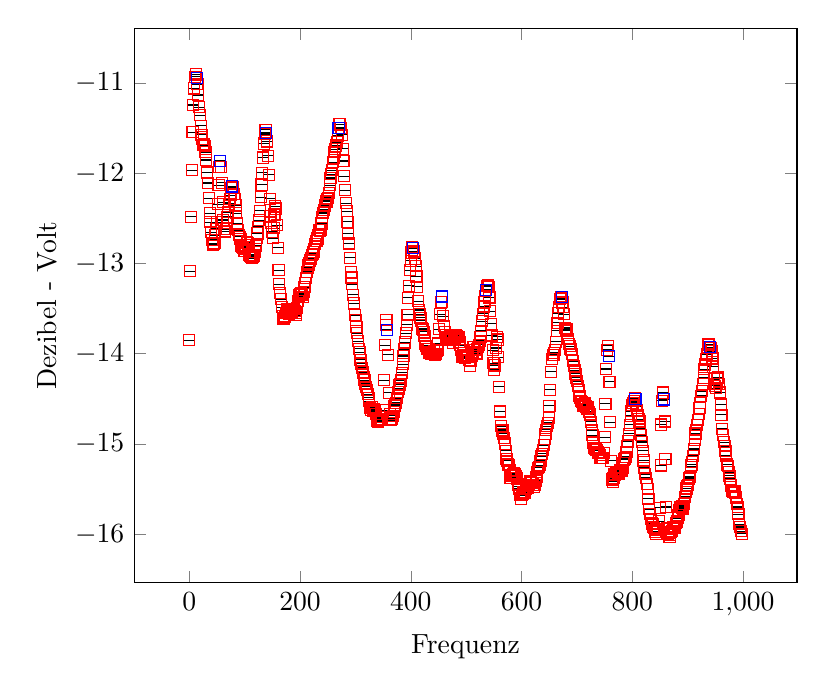
\begin{tikzpicture}
		\pgfplotsset{width=10cm,compat=1.3,legend style={font=\footnotesize}}
		\begin{axis}[xlabel={Frequenz},ylabel={Dezibel - Volt},legend cell align=left,legend pos=north west]
		
\addplot+[only marks,color=red,mark=square,error bars/.cd,x dir=both,x explicit,y dir=both,y explicit,error bar style={color=black}] table[x=X,y=Y,x error=xerror,y error=yerror,row sep=\\]{
			X	Y	xerror	yerror	\\
			 0.0 	 -13.848843 	 0 	 0 	\\
			 1.464844 	 -13.084864 	 0 	 0 	\\
			 2.929687 	 -12.482075 	 0 	 0 	\\
			 4.394531 	 -11.965661 	 0 	 0 	\\
			 5.859375 	 -11.546794 	 0 	 0 	\\
			 7.324219 	 -11.244475 	 0 	 0 	\\
			 8.789062 	 -11.060753 	 0 	 0 	\\
			 10.253906 	 -10.930851 	 0 	 0 	\\
			 11.71875 	 -10.905362 	 0 	 0 	\\
			 13.183594 	 -10.945357 	 0 	 0 	\\
			 14.648437 	 -11.015081 	 0 	 0 	\\
			 16.113281 	 -11.133686 	 0 	 0 	\\
			 17.578125 	 -11.268296 	 0 	 0 	\\
			 19.042969 	 -11.358805 	 0 	 0 	\\
			 20.507812 	 -11.472242 	 0 	 0 	\\
			 21.972656 	 -11.572217 	 0 	 0 	\\
			 23.4375 	 -11.621438 	 0 	 0 	\\
			 24.902344 	 -11.691274 	 0 	 0 	\\
			 26.367187 	 -11.680804 	 0 	 0 	\\
			 27.832031 	 -11.699508 	 0 	 0 	\\
			 29.296875 	 -11.7647 	 0 	 0 	\\
			 30.761719 	 -11.852881 	 0 	 0 	\\
			 32.226562 	 -11.99242 	 0 	 0 	\\
			 33.691406 	 -12.107867 	 0 	 0 	\\
			 35.15625 	 -12.275713 	 0 	 0 	\\
			 36.621094 	 -12.441633 	 0 	 0 	\\
			 38.085937 	 -12.54294 	 0 	 0 	\\
			 39.550781 	 -12.651932 	 0 	 0 	\\
			 41.015625 	 -12.737365 	 0 	 0 	\\
			 42.480469 	 -12.788693 	 0 	 0 	\\
			 43.945312 	 -12.777987 	 0 	 0 	\\
			 45.410156 	 -12.77724 	 0 	 0 	\\
			 46.875 	 -12.68664 	 0 	 0 	\\
			 48.339844 	 -12.616001 	 0 	 0 	\\
			 49.804687 	 -12.544291 	 0 	 0 	\\
			 51.269531 	 -12.344349 	 0 	 0 	\\
			 52.734375 	 -12.132418 	 0 	 0 	\\
			 54.199219 	 -11.929949 	 0 	 0 	\\
			 55.664062 	 -11.861673 	 0 	 0 	\\
			 57.128906 	 -11.927901 	 0 	 0 	\\
			 58.59375 	 -12.103909 	 0 	 0 	\\
			 60.058594 	 -12.32203 	 0 	 0 	\\
			 61.523437 	 -12.517847 	 0 	 0 	\\
			 62.988281 	 -12.616468 	 0 	 0 	\\
			 64.453125 	 -12.645748 	 0 	 0 	\\
			 65.917969 	 -12.61736 	 0 	 0 	\\
			 67.382812 	 -12.552704 	 0 	 0 	\\
			 68.847656 	 -12.484294 	 0 	 0 	\\
			 70.3125 	 -12.432589 	 0 	 0 	\\
			 71.777344 	 -12.339848 	 0 	 0 	\\
			 73.242187 	 -12.285835 	 0 	 0 	\\
			 74.707031 	 -12.244226 	 0 	 0 	\\
			 76.171875 	 -12.159871 	 0 	 0 	\\
			 77.636719 	 -12.146492 	 0 	 0 	\\
			 79.101562 	 -12.15427 	 0 	 0 	\\
			 80.566406 	 -12.22811 	 0 	 0 	\\
			 82.03125 	 -12.288702 	 0 	 0 	\\
			 83.496094 	 -12.357264 	 0 	 0 	\\
			 84.960937 	 -12.44275 	 0 	 0 	\\
			 86.425781 	 -12.553677 	 0 	 0 	\\
			 87.890625 	 -12.6296 	 0 	 0 	\\
			 89.355469 	 -12.688173 	 0 	 0 	\\
			 90.820312 	 -12.704946 	 0 	 0 	\\
			 92.285156 	 -12.731203 	 0 	 0 	\\
			 93.75 	 -12.801209 	 0 	 0 	\\
			 95.214844 	 -12.81376 	 0 	 0 	\\
			 96.679687 	 -12.822852 	 0 	 0 	\\
			 98.144531 	 -12.862325 	 0 	 0 	\\
			 99.609375 	 -12.835527 	 0 	 0 	\\
			 101.074219 	 -12.861899 	 0 	 0 	\\
			 102.539062 	 -12.796264 	 0 	 0 	\\
			 104.003906 	 -12.767695 	 0 	 0 	\\
			 105.46875 	 -12.776719 	 0 	 0 	\\
			 106.933594 	 -12.820479 	 0 	 0 	\\
			 108.398437 	 -12.902568 	 0 	 0 	\\
			 109.863281 	 -12.912542 	 0 	 0 	\\
			 111.328125 	 -12.925619 	 0 	 0 	\\
			 112.792969 	 -12.94205 	 0 	 0 	\\
			 114.257812 	 -12.925128 	 0 	 0 	\\
			 115.722656 	 -12.917577 	 0 	 0 	\\
			 117.1875 	 -12.910091 	 0 	 0 	\\
			 118.652344 	 -12.877029 	 0 	 0 	\\
			 120.117187 	 -12.804531 	 0 	 0 	\\
			 121.582031 	 -12.721627 	 0 	 0 	\\
			 123.046875 	 -12.667387 	 0 	 0 	\\
			 124.511719 	 -12.593013 	 0 	 0 	\\
			 125.976562 	 -12.521207 	 0 	 0 	\\
			 127.441406 	 -12.417398 	 0 	 0 	\\
			 128.90625 	 -12.265208 	 0 	 0 	\\
			 130.371094 	 -12.125359 	 0 	 0 	\\
			 131.835937 	 -11.994921 	 0 	 0 	\\
			 133.300781 	 -11.826387 	 0 	 0 	\\
			 134.765625 	 -11.671044 	 0 	 0 	\\
			 136.230469 	 -11.565237 	 0 	 0 	\\
			 137.695312 	 -11.518209 	 0 	 0 	\\
			 139.160156 	 -11.552087 	 0 	 0 	\\
			 140.625 	 -11.648033 	 0 	 0 	\\
			 142.089844 	 -11.807956 	 0 	 0 	\\
			 143.554687 	 -12.018671 	 0 	 0 	\\
			 145.019531 	 -12.281651 	 0 	 0 	\\
			 146.484375 	 -12.478611 	 0 	 0 	\\
			 147.949219 	 -12.546177 	 0 	 0 	\\
			 149.414062 	 -12.648767 	 0 	 0 	\\
			 150.878906 	 -12.717481 	 0 	 0 	\\
			 152.34375 	 -12.60883 	 0 	 0 	\\
			 153.808594 	 -12.45765 	 0 	 0 	\\
			 155.273437 	 -12.368136 	 0 	 0 	\\
			 156.738281 	 -12.391095 	 0 	 0 	\\
			 158.203125 	 -12.574885 	 0 	 0 	\\
			 159.667969 	 -12.825482 	 0 	 0 	\\
			 161.132812 	 -13.075072 	 0 	 0 	\\
			 162.597656 	 -13.229819 	 0 	 0 	\\
			 164.0625 	 -13.330846 	 0 	 0 	\\
			 165.527344 	 -13.396548 	 0 	 0 	\\
			 166.992187 	 -13.48553 	 0 	 0 	\\
			 168.457031 	 -13.585124 	 0 	 0 	\\
			 169.921875 	 -13.610015 	 0 	 0 	\\
			 171.386719 	 -13.605334 	 0 	 0 	\\
			 172.851562 	 -13.591405 	 0 	 0 	\\
			 174.316406 	 -13.544796 	 0 	 0 	\\
			 175.78125 	 -13.542664 	 0 	 0 	\\
			 177.246094 	 -13.510556 	 0 	 0 	\\
			 178.710937 	 -13.52105 	 0 	 0 	\\
			 180.175781 	 -13.553794 	 0 	 0 	\\
			 181.640625 	 -13.548846 	 0 	 0 	\\
			 183.105469 	 -13.544876 	 0 	 0 	\\
			 184.570312 	 -13.54253 	 0 	 0 	\\
			 186.035156 	 -13.513837 	 0 	 0 	\\
			 187.5 	 -13.507518 	 0 	 0 	\\
			 188.964844 	 -13.50047 	 0 	 0 	\\
			 190.429687 	 -13.527512 	 0 	 0 	\\
			 191.894531 	 -13.570786 	 0 	 0 	\\
			 193.359375 	 -13.552947 	 0 	 0 	\\
			 194.824219 	 -13.494712 	 0 	 0 	\\
			 196.289062 	 -13.41887 	 0 	 0 	\\
			 197.753906 	 -13.353909 	 0 	 0 	\\
			 199.21875 	 -13.337684 	 0 	 0 	\\
			 200.683594 	 -13.351425 	 0 	 0 	\\
			 202.148437 	 -13.330976 	 0 	 0 	\\
			 203.613281 	 -13.34627 	 0 	 0 	\\
			 205.078125 	 -13.370569 	 0 	 0 	\\
			 206.542969 	 -13.317163 	 0 	 0 	\\
			 208.007812 	 -13.262286 	 0 	 0 	\\
			 209.472656 	 -13.217603 	 0 	 0 	\\
			 210.9375 	 -13.157769 	 0 	 0 	\\
			 212.402344 	 -13.092333 	 0 	 0 	\\
			 213.867187 	 -13.048602 	 0 	 0 	\\
			 215.332031 	 -13.01314 	 0 	 0 	\\
			 216.796875 	 -12.999195 	 0 	 0 	\\
			 218.261719 	 -12.967447 	 0 	 0 	\\
			 219.726562 	 -12.943947 	 0 	 0 	\\
			 221.191406 	 -12.908824 	 0 	 0 	\\
			 222.65625 	 -12.892823 	 0 	 0 	\\
			 224.121094 	 -12.873651 	 0 	 0 	\\
			 225.585937 	 -12.845595 	 0 	 0 	\\
			 227.050781 	 -12.787115 	 0 	 0 	\\
			 228.515625 	 -12.751273 	 0 	 0 	\\
			 229.980469 	 -12.753224 	 0 	 0 	\\
			 231.445312 	 -12.723715 	 0 	 0 	\\
			 232.910156 	 -12.690077 	 0 	 0 	\\
			 234.375 	 -12.628439 	 0 	 0 	\\
			 235.839844 	 -12.634004 	 0 	 0 	\\
			 237.304687 	 -12.631191 	 0 	 0 	\\
			 238.769531 	 -12.556608 	 0 	 0 	\\
			 240.234375 	 -12.487989 	 0 	 0 	\\
			 241.699219 	 -12.44106 	 0 	 0 	\\
			 243.164062 	 -12.403562 	 0 	 0 	\\
			 244.628906 	 -12.357152 	 0 	 0 	\\
			 246.09375 	 -12.307795 	 0 	 0 	\\
			 247.558594 	 -12.317731 	 0 	 0 	\\
			 249.023437 	 -12.281264 	 0 	 0 	\\
			 250.488281 	 -12.27329 	 0 	 0 	\\
			 251.953125 	 -12.218162 	 0 	 0 	\\
			 253.417969 	 -12.134033 	 0 	 0 	\\
			 254.882812 	 -12.052472 	 0 	 0 	\\
			 256.347656 	 -12.011626 	 0 	 0 	\\
			 257.8125 	 -11.966825 	 0 	 0 	\\
			 259.277344 	 -11.878083 	 0 	 0 	\\
			 260.742187 	 -11.830478 	 0 	 0 	\\
			 262.207031 	 -11.761236 	 0 	 0 	\\
			 263.671875 	 -11.733871 	 0 	 0 	\\
			 265.136719 	 -11.693561 	 0 	 0 	\\
			 266.601562 	 -11.65706 	 0 	 0 	\\
			 268.066406 	 -11.581274 	 0 	 0 	\\
			 269.53125 	 -11.497283 	 0 	 0 	\\
			 270.996094 	 -11.455608 	 0 	 0 	\\
			 272.460937 	 -11.459285 	 0 	 0 	\\
			 273.925781 	 -11.501212 	 0 	 0 	\\
			 275.390625 	 -11.572617 	 0 	 0 	\\
			 276.855469 	 -11.727455 	 0 	 0 	\\
			 278.320312 	 -11.864044 	 0 	 0 	\\
			 279.785156 	 -12.032756 	 0 	 0 	\\
			 281.25 	 -12.188835 	 0 	 0 	\\
			 282.714844 	 -12.331757 	 0 	 0 	\\
			 284.179687 	 -12.420208 	 0 	 0 	\\
			 285.644531 	 -12.53871 	 0 	 0 	\\
			 287.109375 	 -12.671718 	 0 	 0 	\\
			 288.574219 	 -12.778358 	 0 	 0 	\\
			 290.039062 	 -12.93537 	 0 	 0 	\\
			 291.503906 	 -13.090729 	 0 	 0 	\\
			 292.96875 	 -13.155254 	 0 	 0 	\\
			 294.433594 	 -13.231764 	 0 	 0 	\\
			 295.898437 	 -13.346051 	 0 	 0 	\\
			 297.363281 	 -13.442986 	 0 	 0 	\\
			 298.828125 	 -13.570926 	 0 	 0 	\\
			 300.292969 	 -13.628228 	 0 	 0 	\\
			 301.757812 	 -13.707827 	 0 	 0 	\\
			 303.222656 	 -13.771672 	 0 	 0 	\\
			 304.6875 	 -13.86243 	 0 	 0 	\\
			 306.152344 	 -13.943918 	 0 	 0 	\\
			 307.617187 	 -13.982186 	 0 	 0 	\\
			 309.082031 	 -14.064806 	 0 	 0 	\\
			 310.546875 	 -14.108041 	 0 	 0 	\\
			 312.011719 	 -14.155785 	 0 	 0 	\\
			 313.476562 	 -14.207383 	 0 	 0 	\\
			 314.941406 	 -14.259609 	 0 	 0 	\\
			 316.40625 	 -14.295196 	 0 	 0 	\\
			 317.871094 	 -14.331971 	 0 	 0 	\\
			 319.335937 	 -14.366945 	 0 	 0 	\\
			 320.800781 	 -14.399659 	 0 	 0 	\\
			 322.265625 	 -14.448483 	 0 	 0 	\\
			 323.730469 	 -14.488628 	 0 	 0 	\\
			 325.195312 	 -14.527894 	 0 	 0 	\\
			 326.660156 	 -14.602149 	 0 	 0 	\\
			 328.125 	 -14.620625 	 0 	 0 	\\
			 329.589844 	 -14.593219 	 0 	 0 	\\
			 331.054687 	 -14.630564 	 0 	 0 	\\
			 332.519531 	 -14.630167 	 0 	 0 	\\
			 333.984375 	 -14.608939 	 0 	 0 	\\
			 335.449219 	 -14.636128 	 0 	 0 	\\
			 336.914062 	 -14.667382 	 0 	 0 	\\
			 338.378906 	 -14.725865 	 0 	 0 	\\
			 339.84375 	 -14.742405 	 0 	 0 	\\
			 341.308594 	 -14.755925 	 0 	 0 	\\
			 342.773437 	 -14.733687 	 0 	 0 	\\
			 344.238281 	 -14.720973 	 0 	 0 	\\
			 345.703125 	 -14.734243 	 0 	 0 	\\
			 347.167969 	 -14.721421 	 0 	 0 	\\
			 348.632812 	 -14.700672 	 0 	 0 	\\
			 350.097656 	 -14.624208 	 0 	 0 	\\
			 351.5625 	 -14.293939 	 0 	 0 	\\
			 353.027344 	 -13.905712 	 0 	 0 	\\
			 354.492187 	 -13.677462 	 0 	 0 	\\
			 355.957031 	 -13.621806 	 0 	 0 	\\
			 357.421875 	 -13.733462 	 0 	 0 	\\
			 358.886719 	 -14.009808 	 0 	 0 	\\
			 360.351562 	 -14.433584 	 0 	 0 	\\
			 361.816406 	 -14.665124 	 0 	 0 	\\
			 363.28125 	 -14.717876 	 0 	 0 	\\
			 364.746094 	 -14.737621 	 0 	 0 	\\
			 366.210937 	 -14.718402 	 0 	 0 	\\
			 367.675781 	 -14.686362 	 0 	 0 	\\
			 369.140625 	 -14.64979 	 0 	 0 	\\
			 370.605469 	 -14.578752 	 0 	 0 	\\
			 372.070312 	 -14.563558 	 0 	 0 	\\
			 373.535156 	 -14.541807 	 0 	 0 	\\
			 375.0 	 -14.491673 	 0 	 0 	\\
			 376.464844 	 -14.426708 	 0 	 0 	\\
			 377.929687 	 -14.385033 	 0 	 0 	\\
			 379.394531 	 -14.344742 	 0 	 0 	\\
			 380.859375 	 -14.338758 	 0 	 0 	\\
			 382.324219 	 -14.297165 	 0 	 0 	\\
			 383.789062 	 -14.21249 	 0 	 0 	\\
			 385.253906 	 -14.117258 	 0 	 0 	\\
			 386.71875 	 -14.024889 	 0 	 0 	\\
			 388.183594 	 -13.94739 	 0 	 0 	\\
			 389.648437 	 -13.874926 	 0 	 0 	\\
			 391.113281 	 -13.773478 	 0 	 0 	\\
			 392.578125 	 -13.67769 	 0 	 0 	\\
			 394.042969 	 -13.566935 	 0 	 0 	\\
			 395.507812 	 -13.380635 	 0 	 0 	\\
			 396.972656 	 -13.246249 	 0 	 0 	\\
			 398.4375 	 -13.075774 	 0 	 0 	\\
			 399.902344 	 -12.971014 	 0 	 0 	\\
			 401.367187 	 -12.878876 	 0 	 0 	\\
			 402.832031 	 -12.8139 	 0 	 0 	\\
			 404.296875 	 -12.828142 	 0 	 0 	\\
			 405.761719 	 -12.866463 	 0 	 0 	\\
			 407.226562 	 -12.945724 	 0 	 0 	\\
			 408.691406 	 -13.031688 	 0 	 0 	\\
			 410.15625 	 -13.14485 	 0 	 0 	\\
			 411.621094 	 -13.257695 	 0 	 0 	\\
			 413.085937 	 -13.418539 	 0 	 0 	\\
			 414.550781 	 -13.515303 	 0 	 0 	\\
			 416.015625 	 -13.560336 	 0 	 0 	\\
			 417.480469 	 -13.602901 	 0 	 0 	\\
			 418.945312 	 -13.633774 	 0 	 0 	\\
			 420.410156 	 -13.721082 	 0 	 0 	\\
			 421.875 	 -13.732183 	 0 	 0 	\\
			 423.339844 	 -13.758321 	 0 	 0 	\\
			 424.804687 	 -13.801134 	 0 	 0 	\\
			 426.269531 	 -13.888743 	 0 	 0 	\\
			 427.734375 	 -13.913864 	 0 	 0 	\\
			 429.199219 	 -13.943489 	 0 	 0 	\\
			 430.664062 	 -13.944173 	 0 	 0 	\\
			 432.128906 	 -13.951193 	 0 	 0 	\\
			 433.59375 	 -13.988607 	 0 	 0 	\\
			 435.058594 	 -13.984307 	 0 	 0 	\\
			 436.523437 	 -14.003439 	 0 	 0 	\\
			 437.988281 	 -14.003711 	 0 	 0 	\\
			 439.453125 	 -14.003144 	 0 	 0 	\\
			 440.917969 	 -13.999819 	 0 	 0 	\\
			 442.382812 	 -13.974069 	 0 	 0 	\\
			 443.847656 	 -14.010213 	 0 	 0 	\\
			 445.3125 	 -14.005608 	 0 	 0 	\\
			 446.777344 	 -13.972788 	 0 	 0 	\\
			 448.242187 	 -13.957638 	 0 	 0 	\\
			 449.707031 	 -13.886552 	 0 	 0 	\\
			 451.171875 	 -13.726927 	 0 	 0 	\\
			 452.636719 	 -13.564186 	 0 	 0 	\\
			 454.101562 	 -13.431608 	 0 	 0 	\\
			 455.566406 	 -13.365859 	 0 	 0 	\\
			 457.03125 	 -13.423494 	 0 	 0 	\\
			 458.496094 	 -13.582422 	 0 	 0 	\\
			 459.960937 	 -13.695712 	 0 	 0 	\\
			 461.425781 	 -13.759894 	 0 	 0 	\\
			 462.890625 	 -13.793842 	 0 	 0 	\\
			 464.355469 	 -13.827708 	 0 	 0 	\\
			 465.820312 	 -13.83685 	 0 	 0 	\\
			 467.285156 	 -13.830297 	 0 	 0 	\\
			 468.75 	 -13.81644 	 0 	 0 	\\
			 470.214844 	 -13.845641 	 0 	 0 	\\
			 471.679687 	 -13.829206 	 0 	 0 	\\
			 473.144531 	 -13.803917 	 0 	 0 	\\
			 474.609375 	 -13.849516 	 0 	 0 	\\
			 476.074219 	 -13.880946 	 0 	 0 	\\
			 477.539062 	 -13.848585 	 0 	 0 	\\
			 479.003906 	 -13.831017 	 0 	 0 	\\
			 480.46875 	 -13.805676 	 0 	 0 	\\
			 481.933594 	 -13.791267 	 0 	 0 	\\
			 483.398437 	 -13.800226 	 0 	 0 	\\
			 484.863281 	 -13.818996 	 0 	 0 	\\
			 486.328125 	 -13.818732 	 0 	 0 	\\
			 487.792969 	 -13.86874 	 0 	 0 	\\
			 489.257812 	 -13.907663 	 0 	 0 	\\
			 490.722656 	 -13.961497 	 0 	 0 	\\
			 492.1875 	 -14.02978 	 0 	 0 	\\
			 493.652344 	 -14.019824 	 0 	 0 	\\
			 495.117187 	 -14.010858 	 0 	 0 	\\
			 496.582031 	 -14.030786 	 0 	 0 	\\
			 498.046875 	 -14.049811 	 0 	 0 	\\
			 499.511719 	 -14.020986 	 0 	 0 	\\
			 500.976562 	 -14.028292 	 0 	 0 	\\
			 502.441406 	 -14.02857 	 0 	 0 	\\
			 503.90625 	 -14.038276 	 0 	 0 	\\
			 505.371094 	 -14.073226 	 0 	 0 	\\
			 506.835937 	 -14.139538 	 0 	 0 	\\
			 508.300781 	 -14.082113 	 0 	 0 	\\
			 509.765625 	 -14.022043 	 0 	 0 	\\
			 511.230469 	 -13.977014 	 0 	 0 	\\
			 512.695312 	 -13.928044 	 0 	 0 	\\
			 514.160156 	 -13.927798 	 0 	 0 	\\
			 515.625 	 -13.961398 	 0 	 0 	\\
			 517.089844 	 -13.9973 	 0 	 0 	\\
			 518.554687 	 -14.001409 	 0 	 0 	\\
			 520.019531 	 -13.952327 	 0 	 0 	\\
			 521.484375 	 -13.921497 	 0 	 0 	\\
			 522.949219 	 -13.899399 	 0 	 0 	\\
			 524.414062 	 -13.856237 	 0 	 0 	\\
			 525.878906 	 -13.811698 	 0 	 0 	\\
			 527.34375 	 -13.74543 	 0 	 0 	\\
			 528.808594 	 -13.640151 	 0 	 0 	\\
			 530.273437 	 -13.558892 	 0 	 0 	\\
			 531.738281 	 -13.476128 	 0 	 0 	\\
			 533.203125 	 -13.424129 	 0 	 0 	\\
			 534.667969 	 -13.361391 	 0 	 0 	\\
			 536.132812 	 -13.290147 	 0 	 0 	\\
			 537.597656 	 -13.249411 	 0 	 0 	\\
			 539.0625 	 -13.243973 	 0 	 0 	\\
			 540.527344 	 -13.258794 	 0 	 0 	\\
			 541.992187 	 -13.376017 	 0 	 0 	\\
			 543.457031 	 -13.53083 	 0 	 0 	\\
			 544.921875 	 -13.669553 	 0 	 0 	\\
			 546.386719 	 -13.797888 	 0 	 0 	\\
			 547.851562 	 -13.962575 	 0 	 0 	\\
			 549.316406 	 -14.103863 	 0 	 0 	\\
			 550.78125 	 -14.175672 	 0 	 0 	\\
			 552.246094 	 -14.129969 	 0 	 0 	\\
			 553.710937 	 -13.935889 	 0 	 0 	\\
			 555.175781 	 -13.812741 	 0 	 0 	\\
			 556.640625 	 -13.842486 	 0 	 0 	\\
			 558.105469 	 -14.0394 	 0 	 0 	\\
			 559.570312 	 -14.36572 	 0 	 0 	\\
			 561.035156 	 -14.639869 	 0 	 0 	\\
			 562.5 	 -14.803625 	 0 	 0 	\\
			 563.964844 	 -14.852777 	 0 	 0 	\\
			 565.429687 	 -14.841215 	 0 	 0 	\\
			 566.894531 	 -14.885598 	 0 	 0 	\\
			 568.359375 	 -14.93465 	 0 	 0 	\\
			 569.824219 	 -14.995193 	 0 	 0 	\\
			 571.289062 	 -15.075983 	 0 	 0 	\\
			 572.753906 	 -15.162594 	 0 	 0 	\\
			 574.21875 	 -15.184264 	 0 	 0 	\\
			 575.683594 	 -15.227345 	 0 	 0 	\\
			 577.148437 	 -15.232505 	 0 	 0 	\\
			 578.613281 	 -15.293614 	 0 	 0 	\\
			 580.078125 	 -15.372789 	 0 	 0 	\\
			 581.542969 	 -15.356886 	 0 	 0 	\\
			 583.007812 	 -15.342438 	 0 	 0 	\\
			 584.472656 	 -15.331652 	 0 	 0 	\\
			 585.9375 	 -15.325742 	 0 	 0 	\\
			 587.402344 	 -15.342131 	 0 	 0 	\\
			 588.867187 	 -15.331516 	 0 	 0 	\\
			 590.332031 	 -15.355327 	 0 	 0 	\\
			 591.796875 	 -15.381597 	 0 	 0 	\\
			 593.261719 	 -15.448496 	 0 	 0 	\\
			 594.726562 	 -15.472652 	 0 	 0 	\\
			 596.191406 	 -15.492994 	 0 	 0 	\\
			 597.65625 	 -15.566356 	 0 	 0 	\\
			 599.121094 	 -15.605995 	 0 	 0 	\\
			 600.585937 	 -15.568733 	 0 	 0 	\\
			 602.050781 	 -15.554772 	 0 	 0 	\\
			 603.515625 	 -15.53828 	 0 	 0 	\\
			 604.980469 	 -15.538965 	 0 	 0 	\\
			 606.445312 	 -15.536983 	 0 	 0 	\\
			 607.910156 	 -15.502813 	 0 	 0 	\\
			 609.375 	 -15.469022 	 0 	 0 	\\
			 610.839844 	 -15.483412 	 0 	 0 	\\
			 612.304687 	 -15.461215 	 0 	 0 	\\
			 613.769531 	 -15.456343 	 0 	 0 	\\
			 615.234375 	 -15.407683 	 0 	 0 	\\
			 616.699219 	 -15.420788 	 0 	 0 	\\
			 618.164062 	 -15.43605 	 0 	 0 	\\
			 619.628906 	 -15.432121 	 0 	 0 	\\
			 621.09375 	 -15.455558 	 0 	 0 	\\
			 622.558594 	 -15.478613 	 0 	 0 	\\
			 624.023437 	 -15.449878 	 0 	 0 	\\
			 625.488281 	 -15.404584 	 0 	 0 	\\
			 626.953125 	 -15.368659 	 0 	 0 	\\
			 628.417969 	 -15.307146 	 0 	 0 	\\
			 629.882812 	 -15.26498 	 0 	 0 	\\
			 631.347656 	 -15.254311 	 0 	 0 	\\
			 632.8125 	 -15.235234 	 0 	 0 	\\
			 634.277344 	 -15.186217 	 0 	 0 	\\
			 635.742187 	 -15.138761 	 0 	 0 	\\
			 637.207031 	 -15.106788 	 0 	 0 	\\
			 638.671875 	 -15.069259 	 0 	 0 	\\
			 640.136719 	 -15.015678 	 0 	 0 	\\
			 641.601562 	 -14.946323 	 0 	 0 	\\
			 643.066406 	 -14.888166 	 0 	 0 	\\
			 644.53125 	 -14.841577 	 0 	 0 	\\
			 645.996094 	 -14.80279 	 0 	 0 	\\
			 647.460937 	 -14.763057 	 0 	 0 	\\
			 648.925781 	 -14.707606 	 0 	 0 	\\
			 650.390625 	 -14.576478 	 0 	 0 	\\
			 651.855469 	 -14.399101 	 0 	 0 	\\
			 653.320312 	 -14.201233 	 0 	 0 	\\
			 654.785156 	 -14.05587 	 0 	 0 	\\
			 656.25 	 -14.01161 	 0 	 0 	\\
			 657.714844 	 -14.015326 	 0 	 0 	\\
			 659.179687 	 -13.989563 	 0 	 0 	\\
			 660.644531 	 -13.957742 	 0 	 0 	\\
			 662.109375 	 -13.86798 	 0 	 0 	\\
			 663.574219 	 -13.74568 	 0 	 0 	\\
			 665.039062 	 -13.655993 	 0 	 0 	\\
			 666.503906 	 -13.551404 	 0 	 0 	\\
			 667.96875 	 -13.482943 	 0 	 0 	\\
			 669.433594 	 -13.394012 	 0 	 0 	\\
			 670.898437 	 -13.376683 	 0 	 0 	\\
			 672.363281 	 -13.373598 	 0 	 0 	\\
			 673.828125 	 -13.432512 	 0 	 0 	\\
			 675.292969 	 -13.483224 	 0 	 0 	\\
			 676.757812 	 -13.563242 	 0 	 0 	\\
			 678.222656 	 -13.713531 	 0 	 0 	\\
			 679.6875 	 -13.731859 	 0 	 0 	\\
			 681.152344 	 -13.725105 	 0 	 0 	\\
			 682.617187 	 -13.746216 	 0 	 0 	\\
			 684.082031 	 -13.834937 	 0 	 0 	\\
			 685.546875 	 -13.892766 	 0 	 0 	\\
			 687.011719 	 -13.917761 	 0 	 0 	\\
			 688.476562 	 -13.944634 	 0 	 0 	\\
			 689.941406 	 -13.954781 	 0 	 0 	\\
			 691.40625 	 -14.00583 	 0 	 0 	\\
			 692.871094 	 -14.080033 	 0 	 0 	\\
			 694.335937 	 -14.13577 	 0 	 0 	\\
			 695.800781 	 -14.186631 	 0 	 0 	\\
			 697.265625 	 -14.221995 	 0 	 0 	\\
			 698.730469 	 -14.264764 	 0 	 0 	\\
			 700.195312 	 -14.304014 	 0 	 0 	\\
			 701.660156 	 -14.358989 	 0 	 0 	\\
			 703.125 	 -14.406108 	 0 	 0 	\\
			 704.589844 	 -14.467628 	 0 	 0 	\\
			 706.054687 	 -14.492406 	 0 	 0 	\\
			 707.519531 	 -14.52735 	 0 	 0 	\\
			 708.984375 	 -14.533796 	 0 	 0 	\\
			 710.449219 	 -14.557829 	 0 	 0 	\\
			 711.914062 	 -14.576191 	 0 	 0 	\\
			 713.378906 	 -14.564985 	 0 	 0 	\\
			 714.84375 	 -14.551908 	 0 	 0 	\\
			 716.308594 	 -14.585457 	 0 	 0 	\\
			 717.773437 	 -14.60963 	 0 	 0 	\\
			 719.238281 	 -14.594293 	 0 	 0 	\\
			 720.703125 	 -14.598125 	 0 	 0 	\\
			 722.167969 	 -14.644541 	 0 	 0 	\\
			 723.632812 	 -14.672808 	 0 	 0 	\\
			 725.097656 	 -14.752396 	 0 	 0 	\\
			 726.5625 	 -14.851145 	 0 	 0 	\\
			 728.027344 	 -14.90107 	 0 	 0 	\\
			 729.492187 	 -14.983686 	 0 	 0 	\\
			 730.957031 	 -15.045944 	 0 	 0 	\\
			 732.421875 	 -15.059546 	 0 	 0 	\\
			 733.886719 	 -15.05426 	 0 	 0 	\\
			 735.351562 	 -15.064187 	 0 	 0 	\\
			 736.816406 	 -15.066898 	 0 	 0 	\\
			 738.28125 	 -15.093438 	 0 	 0 	\\
			 739.746094 	 -15.100656 	 0 	 0 	\\
			 741.210937 	 -15.12522 	 0 	 0 	\\
			 742.675781 	 -15.158319 	 0 	 0 	\\
			 744.140625 	 -15.157933 	 0 	 0 	\\
			 745.605469 	 -15.158154 	 0 	 0 	\\
			 747.070312 	 -15.158847 	 0 	 0 	\\
			 748.535156 	 -15.099766 	 0 	 0 	\\
			 750.0 	 -14.92643 	 0 	 0 	\\
			 751.464844 	 -14.552396 	 0 	 0 	\\
			 752.929687 	 -14.1692 	 0 	 0 	\\
			 754.394531 	 -13.958285 	 0 	 0 	\\
			 755.859375 	 -13.911774 	 0 	 0 	\\
			 757.324219 	 -14.028664 	 0 	 0 	\\
			 758.789062 	 -14.312077 	 0 	 0 	\\
			 760.253906 	 -14.760731 	 0 	 0 	\\
			 761.71875 	 -15.184678 	 0 	 0 	\\
			 763.183594 	 -15.392624 	 0 	 0 	\\
			 764.648437 	 -15.418165 	 0 	 0 	\\
			 766.113281 	 -15.377866 	 0 	 0 	\\
			 767.578125 	 -15.336439 	 0 	 0 	\\
			 769.042969 	 -15.34766 	 0 	 0 	\\
			 770.507812 	 -15.309141 	 0 	 0 	\\
			 771.972656 	 -15.309903 	 0 	 0 	\\
			 773.4375 	 -15.321543 	 0 	 0 	\\
			 774.902344 	 -15.330109 	 0 	 0 	\\
			 776.367187 	 -15.306724 	 0 	 0 	\\
			 777.832031 	 -15.288806 	 0 	 0 	\\
			 779.296875 	 -15.301909 	 0 	 0 	\\
			 780.761719 	 -15.295229 	 0 	 0 	\\
			 782.226562 	 -15.27009 	 0 	 0 	\\
			 783.691406 	 -15.208692 	 0 	 0 	\\
			 785.15625 	 -15.171063 	 0 	 0 	\\
			 786.621094 	 -15.161349 	 0 	 0 	\\
			 788.085937 	 -15.1401 	 0 	 0 	\\
			 789.550781 	 -15.091379 	 0 	 0 	\\
			 791.015625 	 -15.026564 	 0 	 0 	\\
			 792.480469 	 -14.972059 	 0 	 0 	\\
			 793.945312 	 -14.887531 	 0 	 0 	\\
			 795.410156 	 -14.786565 	 0 	 0 	\\
			 796.875 	 -14.689001 	 0 	 0 	\\
			 798.339844 	 -14.635184 	 0 	 0 	\\
			 799.804687 	 -14.567341 	 0 	 0 	\\
			 801.269531 	 -14.541805 	 0 	 0 	\\
			 802.734375 	 -14.523753 	 0 	 0 	\\
			 804.199219 	 -14.48997 	 0 	 0 	\\
			 805.664062 	 -14.504683 	 0 	 0 	\\
			 807.128906 	 -14.57874 	 0 	 0 	\\
			 808.59375 	 -14.629734 	 0 	 0 	\\
			 810.058594 	 -14.684223 	 0 	 0 	\\
			 811.523437 	 -14.72411 	 0 	 0 	\\
			 812.988281 	 -14.750403 	 0 	 0 	\\
			 814.453125 	 -14.831126 	 0 	 0 	\\
			 815.917969 	 -14.904781 	 0 	 0 	\\
			 817.382812 	 -14.977625 	 0 	 0 	\\
			 818.847656 	 -15.07545 	 0 	 0 	\\
			 820.3125 	 -15.182081 	 0 	 0 	\\
			 821.777344 	 -15.261506 	 0 	 0 	\\
			 823.242187 	 -15.335604 	 0 	 0 	\\
			 824.707031 	 -15.375717 	 0 	 0 	\\
			 826.171875 	 -15.442172 	 0 	 0 	\\
			 827.636719 	 -15.500808 	 0 	 0 	\\
			 829.101562 	 -15.608633 	 0 	 0 	\\
			 830.566406 	 -15.724411 	 0 	 0 	\\
			 832.03125 	 -15.778374 	 0 	 0 	\\
			 833.496094 	 -15.832983 	 0 	 0 	\\
			 834.960937 	 -15.881127 	 0 	 0 	\\
			 836.425781 	 -15.888403 	 0 	 0 	\\
			 837.890625 	 -15.916879 	 0 	 0 	\\
			 839.355469 	 -15.93463 	 0 	 0 	\\
			 840.820312 	 -15.969865 	 0 	 0 	\\
			 842.285156 	 -15.994647 	 0 	 0 	\\
			 843.75 	 -15.943043 	 0 	 0 	\\
			 845.214844 	 -15.950734 	 0 	 0 	\\
			 846.679687 	 -15.938186 	 0 	 0 	\\
			 848.144531 	 -15.857123 	 0 	 0 	\\
			 849.609375 	 -15.706494 	 0 	 0 	\\
			 851.074219 	 -15.237861 	 0 	 0 	\\
			 852.539062 	 -14.784414 	 0 	 0 	\\
			 854.003906 	 -14.521018 	 0 	 0 	\\
			 855.46875 	 -14.430327 	 0 	 0 	\\
			 856.933594 	 -14.506615 	 0 	 0 	\\
			 858.398437 	 -14.750749 	 0 	 0 	\\
			 859.863281 	 -15.167859 	 0 	 0 	\\
			 861.328125 	 -15.698378 	 0 	 0 	\\
			 862.792969 	 -15.937158 	 0 	 0 	\\
			 864.257812 	 -15.996637 	 0 	 0 	\\
			 865.722656 	 -15.98979 	 0 	 0 	\\
			 867.1875 	 -16.026136 	 0 	 0 	\\
			 868.652344 	 -16.006728 	 0 	 0 	\\
			 870.117187 	 -15.977865 	 0 	 0 	\\
			 871.582031 	 -15.966749 	 0 	 0 	\\
			 873.046875 	 -15.923391 	 0 	 0 	\\
			 874.511719 	 -15.932359 	 0 	 0 	\\
			 875.976562 	 -15.931909 	 0 	 0 	\\
			 877.441406 	 -15.925212 	 0 	 0 	\\
			 878.90625 	 -15.876147 	 0 	 0 	\\
			 880.371094 	 -15.858563 	 0 	 0 	\\
			 881.835937 	 -15.824195 	 0 	 0 	\\
			 883.300781 	 -15.790751 	 0 	 0 	\\
			 884.765625 	 -15.73282 	 0 	 0 	\\
			 886.230469 	 -15.697337 	 0 	 0 	\\
			 887.695312 	 -15.69995 	 0 	 0 	\\
			 889.160156 	 -15.708749 	 0 	 0 	\\
			 890.625 	 -15.686311 	 0 	 0 	\\
			 892.089844 	 -15.716433 	 0 	 0 	\\
			 893.554687 	 -15.665769 	 0 	 0 	\\
			 895.019531 	 -15.583663 	 0 	 0 	\\
			 896.484375 	 -15.531006 	 0 	 0 	\\
			 897.949219 	 -15.492765 	 0 	 0 	\\
			 899.414062 	 -15.469691 	 0 	 0 	\\
			 900.878906 	 -15.453538 	 0 	 0 	\\
			 902.34375 	 -15.382501 	 0 	 0 	\\
			 903.808594 	 -15.366147 	 0 	 0 	\\
			 905.273437 	 -15.253802 	 0 	 0 	\\
			 906.738281 	 -15.228529 	 0 	 0 	\\
			 908.203125 	 -15.194991 	 0 	 0 	\\
			 909.667969 	 -15.130339 	 0 	 0 	\\
			 911.132812 	 -15.055083 	 0 	 0 	\\
			 912.597656 	 -14.951272 	 0 	 0 	\\
			 914.0625 	 -14.883529 	 0 	 0 	\\
			 915.527344 	 -14.843739 	 0 	 0 	\\
			 916.992187 	 -14.787547 	 0 	 0 	\\
			 918.457031 	 -14.732906 	 0 	 0 	\\
			 919.921875 	 -14.671104 	 0 	 0 	\\
			 921.386719 	 -14.602968 	 0 	 0 	\\
			 922.851562 	 -14.544416 	 0 	 0 	\\
			 924.316406 	 -14.465856 	 0 	 0 	\\
			 925.78125 	 -14.417382 	 0 	 0 	\\
			 927.246094 	 -14.333243 	 0 	 0 	\\
			 928.710937 	 -14.265049 	 0 	 0 	\\
			 930.175781 	 -14.173132 	 0 	 0 	\\
			 931.640625 	 -14.11998 	 0 	 0 	\\
			 933.105469 	 -14.063228 	 0 	 0 	\\
			 934.570312 	 -14.009239 	 0 	 0 	\\
			 936.035156 	 -13.929794 	 0 	 0 	\\
			 937.5 	 -13.897684 	 0 	 0 	\\
			 938.964844 	 -13.903076 	 0 	 0 	\\
			 940.429687 	 -13.92639 	 0 	 0 	\\
			 941.894531 	 -13.938956 	 0 	 0 	\\
			 943.359375 	 -13.970751 	 0 	 0 	\\
			 944.824219 	 -14.052549 	 0 	 0 	\\
			 946.289062 	 -14.14161 	 0 	 0 	\\
			 947.753906 	 -14.280235 	 0 	 0 	\\
			 949.21875 	 -14.35463 	 0 	 0 	\\
			 950.683594 	 -14.382016 	 0 	 0 	\\
			 952.148437 	 -14.339008 	 0 	 0 	\\
			 953.613281 	 -14.279057 	 0 	 0 	\\
			 955.078125 	 -14.263344 	 0 	 0 	\\
			 956.542969 	 -14.334046 	 0 	 0 	\\
			 958.007812 	 -14.429471 	 0 	 0 	\\
			 959.472656 	 -14.562532 	 0 	 0 	\\
			 960.9375 	 -14.677482 	 0 	 0 	\\
			 962.402344 	 -14.83028 	 0 	 0 	\\
			 963.867187 	 -14.898317 	 0 	 0 	\\
			 965.332031 	 -14.979098 	 0 	 0 	\\
			 966.796875 	 -15.024695 	 0 	 0 	\\
			 968.261719 	 -15.074795 	 0 	 0 	\\
			 969.726562 	 -15.131465 	 0 	 0 	\\
			 971.191406 	 -15.228137 	 0 	 0 	\\
			 972.65625 	 -15.246065 	 0 	 0 	\\
			 974.121094 	 -15.310705 	 0 	 0 	\\
			 975.585937 	 -15.35391 	 0 	 0 	\\
			 977.050781 	 -15.386969 	 0 	 0 	\\
			 978.515625 	 -15.458913 	 0 	 0 	\\
			 979.980469 	 -15.517785 	 0 	 0 	\\
			 981.445312 	 -15.534356 	 0 	 0 	\\
			 982.910156 	 -15.536297 	 0 	 0 	\\
			 984.375 	 -15.525312 	 0 	 0 	\\
			 985.839844 	 -15.541296 	 0 	 0 	\\
			 987.304687 	 -15.5928 	 0 	 0 	\\
			 988.769531 	 -15.661136 	 0 	 0 	\\
			 990.234375 	 -15.698563 	 0 	 0 	\\
			 991.699219 	 -15.777128 	 0 	 0 	\\
			 993.164062 	 -15.890349 	 0 	 0 	\\
			 994.628906 	 -15.919824 	 0 	 0 	\\
			 996.09375 	 -15.968122 	 0 	 0 	\\
			 997.558594 	 -15.994696 	 0 	 0 	\\
		};
		% \addlegendentry{Messpunkte Datensatz 0}

\addplot+[only marks,color=blue,mark=square,error bars/.cd,x dir=both,x explicit,y dir=both,y explicit,error bar style={color=black}] table[x=X,y=Y,x error=xerror,y error=yerror,row sep=\\]{
			X	Y	xerror	yerror	\\
			 13.183594 	 -10.945357 	 0 	 0 	\\
			 55.664062 	 -11.861673 	 0 	 0 	\\
			 77.636719 	 -12.146492 	 0 	 0 	\\
			 139.160156 	 -11.552087 	 0 	 0 	\\
			 269.53125 	 -11.497283 	 0 	 0 	\\
			 357.421875 	 -13.733462 	 0 	 0 	\\
			 404.296875 	 -12.828142 	 0 	 0 	\\
			 455.566406 	 -13.365859 	 0 	 0 	\\
			 536.132812 	 -13.290147 	 0 	 0 	\\
			 672.363281 	 -13.373598 	 0 	 0 	\\
			 757.324219 	 -14.028664 	 0 	 0 	\\
			 805.664062 	 -14.504683 	 0 	 0 	\\
			 856.933594 	 -14.506615 	 0 	 0 	\\
			 940.429687 	 -13.92639 	 0 	 0 	\\
		};
		% \addlegendentry{Messpunkte Datensatz 1}

		\end{axis}
		\end{tikzpicture}
	\caption{Umgebung}
	\label{fig:Umgebungsmessung}
\end{figure}

        
\end{document}